\documentclass[twoside]{book}

% Packages required by doxygen
\usepackage{fixltx2e}
\usepackage{calc}
\usepackage{doxygen}
\usepackage[export]{adjustbox} % also loads graphicx
\usepackage{graphicx}
\usepackage[utf8]{inputenc}
\usepackage{makeidx}
\usepackage{multicol}
\usepackage{multirow}
\PassOptionsToPackage{warn}{textcomp}
\usepackage{textcomp}
\usepackage[nointegrals]{wasysym}
\usepackage[table]{xcolor}

% NLS support packages
\usepackage[ngerman]{babel}

% Font selection
\usepackage[T1]{fontenc}
\usepackage[scaled=.90]{helvet}
\usepackage{courier}
\usepackage{amssymb}
\usepackage{sectsty}
\renewcommand{\familydefault}{\sfdefault}
\allsectionsfont{%
  \fontseries{bc}\selectfont%
  \color{darkgray}%
}
\renewcommand{\DoxyLabelFont}{%
  \fontseries{bc}\selectfont%
  \color{darkgray}%
}
\newcommand{\+}{\discretionary{\mbox{\scriptsize$\hookleftarrow$}}{}{}}

% Page & text layout
\usepackage{geometry}
\geometry{%
  a4paper,%
  top=2.5cm,%
  bottom=2.5cm,%
  left=2.5cm,%
  right=2.5cm%
}
\tolerance=750
\hfuzz=15pt
\hbadness=750
\setlength{\emergencystretch}{15pt}
\setlength{\parindent}{0cm}
\setlength{\parskip}{3ex plus 2ex minus 2ex}
\makeatletter
\renewcommand{\paragraph}{%
  \@startsection{paragraph}{4}{0ex}{-1.0ex}{1.0ex}{%
    \normalfont\normalsize\bfseries\SS@parafont%
  }%
}
\renewcommand{\subparagraph}{%
  \@startsection{subparagraph}{5}{0ex}{-1.0ex}{1.0ex}{%
    \normalfont\normalsize\bfseries\SS@subparafont%
  }%
}
\makeatother

% Headers & footers
\usepackage{fancyhdr}
\pagestyle{fancyplain}
\fancyhead[LE]{\fancyplain{}{\bfseries\thepage}}
\fancyhead[CE]{\fancyplain{}{}}
\fancyhead[RE]{\fancyplain{}{\bfseries\leftmark}}
\fancyhead[LO]{\fancyplain{}{\bfseries\rightmark}}
\fancyhead[CO]{\fancyplain{}{}}
\fancyhead[RO]{\fancyplain{}{\bfseries\thepage}}
\fancyfoot[LE]{\fancyplain{}{}}
\fancyfoot[CE]{\fancyplain{}{}}
\fancyfoot[RE]{\fancyplain{}{\bfseries\scriptsize Erzeugt von Doxygen }}
\fancyfoot[LO]{\fancyplain{}{\bfseries\scriptsize Erzeugt von Doxygen }}
\fancyfoot[CO]{\fancyplain{}{}}
\fancyfoot[RO]{\fancyplain{}{}}
\renewcommand{\footrulewidth}{0.4pt}
\renewcommand{\chaptermark}[1]{%
  \markboth{#1}{}%
}
\renewcommand{\sectionmark}[1]{%
  \markright{\thesection\ #1}%
}

% Indices & bibliography
\usepackage{natbib}
\usepackage[titles]{tocloft}
\setcounter{tocdepth}{3}
\setcounter{secnumdepth}{5}
\makeindex

% Hyperlinks (required, but should be loaded last)
\usepackage{ifpdf}
\ifpdf
  \usepackage[pdftex,pagebackref=true]{hyperref}
\else
  \usepackage[ps2pdf,pagebackref=true]{hyperref}
\fi
\hypersetup{%
  colorlinks=true,%
  linkcolor=blue,%
  citecolor=blue,%
  unicode%
}

% Custom commands
\newcommand{\clearemptydoublepage}{%
  \newpage{\pagestyle{empty}\cleardoublepage}%
}

\usepackage{caption}
\captionsetup{labelsep=space,justification=centering,font={bf},singlelinecheck=off,skip=4pt,position=top}

%===== C O N T E N T S =====

\begin{document}

% Titlepage & ToC
\hypersetup{pageanchor=false,
             bookmarksnumbered=true,
             pdfencoding=unicode
            }
\pagenumbering{alph}
\begin{titlepage}
\vspace*{7cm}
\begin{center}%
{\Large Abschlussprojekt vollautomatisches Gewächshaus }\\
\vspace*{1cm}
{\large Erzeugt von Doxygen 1.8.13}\\
\end{center}
\end{titlepage}
\clearemptydoublepage
\pagenumbering{roman}
\tableofcontents
\clearemptydoublepage
\pagenumbering{arabic}
\hypersetup{pageanchor=true}

%--- Begin generated contents ---
\chapter{Datei-\/\+Verzeichnis}
\section{Auflistung der Dateien}
Hier folgt die Aufzählung aller Dateien mit einer Kurzbeschreibung\+:\begin{DoxyCompactList}
\item\contentsline{section}{/home/zero/abschlussprojekt/\hyperlink{abschlussprojekt_8c}{abschlussprojekt.\+c} }{\pageref{abschlussprojekt_8c}}{}
\item\contentsline{section}{/home/zero/abschlussprojekt/\hyperlink{make__string_8cpp}{make\+\_\+string.\+cpp} }{\pageref{make__string_8cpp}}{}
\item\contentsline{section}{/home/zero/abschlussprojekt/\hyperlink{make__string_8h}{make\+\_\+string.\+h} }{\pageref{make__string_8h}}{}
\item\contentsline{section}{/home/zero/abschlussprojekt/\hyperlink{makros_8h}{makros.\+h} }{\pageref{makros_8h}}{}
\item\contentsline{section}{/home/zero/abschlussprojekt/\hyperlink{pumpe__1_8cpp}{pumpe\+\_\+1.\+cpp} }{\pageref{pumpe__1_8cpp}}{}
\item\contentsline{section}{/home/zero/abschlussprojekt/\hyperlink{pumpe__1_8h}{pumpe\+\_\+1.\+h} }{\pageref{pumpe__1_8h}}{}
\item\contentsline{section}{/home/zero/abschlussprojekt/\hyperlink{pumpe__2_8cpp}{pumpe\+\_\+2.\+cpp} }{\pageref{pumpe__2_8cpp}}{}
\item\contentsline{section}{/home/zero/abschlussprojekt/\hyperlink{pumpe__2_8h}{pumpe\+\_\+2.\+h} }{\pageref{pumpe__2_8h}}{}
\item\contentsline{section}{/home/zero/abschlussprojekt/\hyperlink{tuer__zu_8cpp}{tuer\+\_\+zu.\+cpp} }{\pageref{tuer__zu_8cpp}}{}
\item\contentsline{section}{/home/zero/abschlussprojekt/\hyperlink{tuer__zu_8h}{tuer\+\_\+zu.\+h} }{\pageref{tuer__zu_8h}}{}
\item\contentsline{section}{/home/zero/abschlussprojekt/\hyperlink{update__lcd_8h}{update\+\_\+lcd.\+h} }{\pageref{update__lcd_8h}}{}
\item\contentsline{section}{/home/zero/abschlussprojekt/\hyperlink{update__limits_8cpp}{update\+\_\+limits.\+cpp} }{\pageref{update__limits_8cpp}}{}
\item\contentsline{section}{/home/zero/abschlussprojekt/\hyperlink{update__limits_8h}{update\+\_\+limits.\+h} }{\pageref{update__limits_8h}}{}
\item\contentsline{section}{/home/zero/abschlussprojekt/\hyperlink{update__messwerte_8h}{update\+\_\+messwerte.\+h} }{\pageref{update__messwerte_8h}}{}
\end{DoxyCompactList}

\chapter{Datei-\/\+Dokumentation}
\hypertarget{abschlussprojekt_8c}{}\section{/home/zero/abschlussprojekt/abschlussprojekt.c-\/\+Dateireferenz}
\label{abschlussprojekt_8c}\index{/home/zero/abschlussprojekt/abschlussprojekt.\+c@{/home/zero/abschlussprojekt/abschlussprojekt.\+c}}
{\ttfamily \#include \char`\"{}makros.\+h\char`\"{}}\newline
{\ttfamily \#include \char`\"{}tuer\+\_\+zu.\+h\char`\"{}}\newline
{\ttfamily \#include \char`\"{}pumpe\+\_\+1.\+h\char`\"{}}\newline
{\ttfamily \#include \char`\"{}pumpe\+\_\+2.\+h\char`\"{}}\newline
{\ttfamily \#include \char`\"{}update\+\_\+limits.\+h\char`\"{}}\newline
{\ttfamily \#include \char`\"{}update\+\_\+lcd.\+h\char`\"{}}\newline
{\ttfamily \#include \char`\"{}update\+\_\+messwerte.\+h\char`\"{}}\newline
Include-\/\+Abhängigkeitsdiagramm für abschlussprojekt.\+c\+:
\nopagebreak
\begin{figure}[H]
\begin{center}
\leavevmode
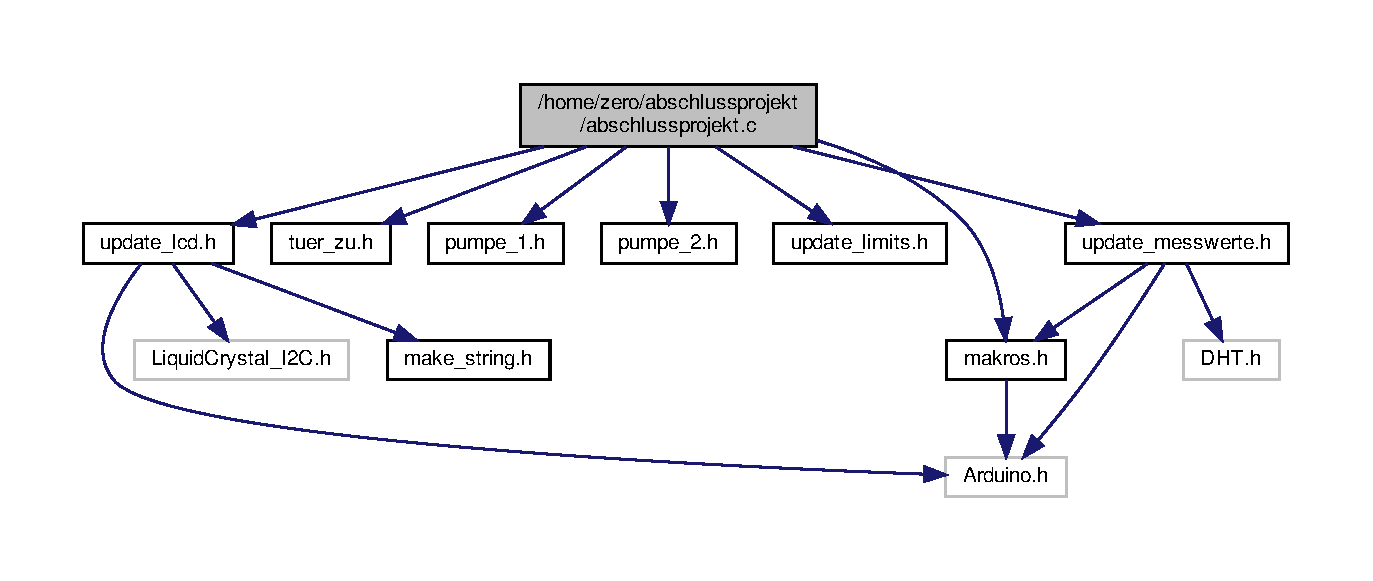
\includegraphics[width=350pt]{abschlussprojekt_8c__incl}
\end{center}
\end{figure}
\subsection*{Funktionen}
\begin{DoxyCompactItemize}
\item 
void \hyperlink{abschlussprojekt_8c_a4fc01d736fe50cf5b977f755b675f11d}{setup} ()
\item 
void \hyperlink{abschlussprojekt_8c_afe461d27b9c48d5921c00d521181f12f}{loop} ()
\end{DoxyCompactItemize}
\subsection*{Variablen}
\begin{DoxyCompactItemize}
\item 
unsigned long \hyperlink{abschlussprojekt_8c_a34dde2eacd6bcd6c70d2717074e5422e}{t0\+\_\+temperaturmessung}
\item 
unsigned long \hyperlink{abschlussprojekt_8c_a8db8552a3060b9b4636a9f4844125b5e}{dt\+\_\+temperaturmessung\+\_\+ms} = 2000
\item 
unsigned long \hyperlink{abschlussprojekt_8c_a6d6f46738f23818a51a33e54540fc834}{t0\+\_\+display}
\item 
unsigned long \hyperlink{abschlussprojekt_8c_aeb4ea2e27ad59b8b80c07f5d9a501578}{dt\+\_\+display\+\_\+ms} = 2000
\item 
unsigned long \hyperlink{abschlussprojekt_8c_aaf3eaa118947402c939df227b9daad8e}{t0\+\_\+erdfeuchtemessung}
\item 
unsigned long \hyperlink{abschlussprojekt_8c_a5a3210d0676305262c0be06fd27f8a77}{dt\+\_\+erdfeuchtemessung\+\_\+ms} = 5000
\item 
unsigned long \hyperlink{abschlussprojekt_8c_a9ca81fb931b2eb83f3a822a49df8995f}{t0\+\_\+heizung}
\item 
unsigned long \hyperlink{abschlussprojekt_8c_a634f1491bed4b1420222d3532ad6903a}{dt\+\_\+heizung\+\_\+ms} = 5000
\item 
unsigned long \hyperlink{abschlussprojekt_8c_a1cc8e9a2f7e21352f0f123728881ad62}{t0\+\_\+luefter}
\item 
unsigned long \hyperlink{abschlussprojekt_8c_a5ff96735fd161b079af42979f93a463a}{dt\+\_\+luefter\+\_\+ms} = 5000
\item 
unsigned long \hyperlink{abschlussprojekt_8c_ab55c3f7b2994108f2af60557f2c801d2}{t0\+\_\+helligkeit}
\item 
unsigned long \hyperlink{abschlussprojekt_8c_a504a3dfe31ae72c0de653e1f1417aff2}{dt\+\_\+helligkeit\+\_\+ms} = 5000
\item 
int \hyperlink{abschlussprojekt_8c_afa416e7460cf043207be351d750b97fe}{hum\+\_\+erde\+\_\+1\+\_\+adc}
\item 
int \hyperlink{abschlussprojekt_8c_aacdbec939adcfa404b8c42b2e064b110}{hum\+\_\+erde\+\_\+2\+\_\+adc}
\item 
int \hyperlink{abschlussprojekt_8c_ac9fcb87eca48e4002731015e004966ef}{hum\+\_\+luft}
\item 
int \hyperlink{abschlussprojekt_8c_a0e6f058da75dead800f4a33e63586703}{temp\+\_\+luft\+\_\+C}
\item 
int \hyperlink{abschlussprojekt_8c_abb1c509cfb119e70585771234accdc4c}{limit\+\_\+feuchte\+\_\+1\+\_\+adc}
\item 
int \hyperlink{abschlussprojekt_8c_a11941af86181c1d0476b4bad92345dee}{limit\+\_\+feuchte\+\_\+2\+\_\+adc}
\item 
int \hyperlink{abschlussprojekt_8c_a8f0ffb4ec25253a324ab4dac6d3cf1c4}{limit\+\_\+temp\+\_\+adc}
\item 
int \hyperlink{abschlussprojekt_8c_a7af3ab4da71f5b8ce8c0d93640690817}{limit\+\_\+temp\+\_\+C}
\item 
int \hyperlink{abschlussprojekt_8c_a3f6dd9ed3b997c063d7c90a38a69ab3a}{limit\+\_\+luefter\+\_\+adc}
\item 
int \hyperlink{abschlussprojekt_8c_a27d916670e311d9e7881ebdc4807e0f5}{limit\+\_\+luefter\+\_\+C}
\item 
int \hyperlink{abschlussprojekt_8c_aa8909f35a0f963844648169d995f3d0a}{voriger\+\_\+taster}
\item 
int \hyperlink{abschlussprojekt_8c_aec00a17d0e71d1e7f6478babd75d6319}{aktueller\+\_\+taster} = H\+I\+GH
\item 
int \hyperlink{abschlussprojekt_8c_a124b7ae42481bdac66b27838ff061b05}{displ\+\_\+nr} = 0
\end{DoxyCompactItemize}


\subsection{Dokumentation der Funktionen}
\mbox{\Hypertarget{abschlussprojekt_8c_afe461d27b9c48d5921c00d521181f12f}\label{abschlussprojekt_8c_afe461d27b9c48d5921c00d521181f12f}} 
\index{abschlussprojekt.\+c@{abschlussprojekt.\+c}!loop@{loop}}
\index{loop@{loop}!abschlussprojekt.\+c@{abschlussprojekt.\+c}}
\subsubsection{\texorpdfstring{loop()}{loop()}}
{\footnotesize\ttfamily void loop (\begin{DoxyParamCaption}{ }\end{DoxyParamCaption})}



Definiert in Zeile 134 der Datei abschlussprojekt.\+c.

\mbox{\Hypertarget{abschlussprojekt_8c_a4fc01d736fe50cf5b977f755b675f11d}\label{abschlussprojekt_8c_a4fc01d736fe50cf5b977f755b675f11d}} 
\index{abschlussprojekt.\+c@{abschlussprojekt.\+c}!setup@{setup}}
\index{setup@{setup}!abschlussprojekt.\+c@{abschlussprojekt.\+c}}
\subsubsection{\texorpdfstring{setup()}{setup()}}
{\footnotesize\ttfamily void setup (\begin{DoxyParamCaption}{ }\end{DoxyParamCaption})}



Definiert in Zeile 69 der Datei abschlussprojekt.\+c.



\subsection{Variablen-\/\+Dokumentation}
\mbox{\Hypertarget{abschlussprojekt_8c_aec00a17d0e71d1e7f6478babd75d6319}\label{abschlussprojekt_8c_aec00a17d0e71d1e7f6478babd75d6319}} 
\index{abschlussprojekt.\+c@{abschlussprojekt.\+c}!aktueller\+\_\+taster@{aktueller\+\_\+taster}}
\index{aktueller\+\_\+taster@{aktueller\+\_\+taster}!abschlussprojekt.\+c@{abschlussprojekt.\+c}}
\subsubsection{\texorpdfstring{aktueller\+\_\+taster}{aktueller\_taster}}
{\footnotesize\ttfamily int aktueller\+\_\+taster = H\+I\+GH}



Definiert in Zeile 61 der Datei abschlussprojekt.\+c.

\mbox{\Hypertarget{abschlussprojekt_8c_a124b7ae42481bdac66b27838ff061b05}\label{abschlussprojekt_8c_a124b7ae42481bdac66b27838ff061b05}} 
\index{abschlussprojekt.\+c@{abschlussprojekt.\+c}!displ\+\_\+nr@{displ\+\_\+nr}}
\index{displ\+\_\+nr@{displ\+\_\+nr}!abschlussprojekt.\+c@{abschlussprojekt.\+c}}
\subsubsection{\texorpdfstring{displ\+\_\+nr}{displ\_nr}}
{\footnotesize\ttfamily int displ\+\_\+nr = 0}



Definiert in Zeile 64 der Datei abschlussprojekt.\+c.

\mbox{\Hypertarget{abschlussprojekt_8c_aeb4ea2e27ad59b8b80c07f5d9a501578}\label{abschlussprojekt_8c_aeb4ea2e27ad59b8b80c07f5d9a501578}} 
\index{abschlussprojekt.\+c@{abschlussprojekt.\+c}!dt\+\_\+display\+\_\+ms@{dt\+\_\+display\+\_\+ms}}
\index{dt\+\_\+display\+\_\+ms@{dt\+\_\+display\+\_\+ms}!abschlussprojekt.\+c@{abschlussprojekt.\+c}}
\subsubsection{\texorpdfstring{dt\+\_\+display\+\_\+ms}{dt\_display\_ms}}
{\footnotesize\ttfamily unsigned long dt\+\_\+display\+\_\+ms = 2000}



Definiert in Zeile 31 der Datei abschlussprojekt.\+c.

\mbox{\Hypertarget{abschlussprojekt_8c_a5a3210d0676305262c0be06fd27f8a77}\label{abschlussprojekt_8c_a5a3210d0676305262c0be06fd27f8a77}} 
\index{abschlussprojekt.\+c@{abschlussprojekt.\+c}!dt\+\_\+erdfeuchtemessung\+\_\+ms@{dt\+\_\+erdfeuchtemessung\+\_\+ms}}
\index{dt\+\_\+erdfeuchtemessung\+\_\+ms@{dt\+\_\+erdfeuchtemessung\+\_\+ms}!abschlussprojekt.\+c@{abschlussprojekt.\+c}}
\subsubsection{\texorpdfstring{dt\+\_\+erdfeuchtemessung\+\_\+ms}{dt\_erdfeuchtemessung\_ms}}
{\footnotesize\ttfamily unsigned long dt\+\_\+erdfeuchtemessung\+\_\+ms = 5000}



Definiert in Zeile 34 der Datei abschlussprojekt.\+c.

\mbox{\Hypertarget{abschlussprojekt_8c_a634f1491bed4b1420222d3532ad6903a}\label{abschlussprojekt_8c_a634f1491bed4b1420222d3532ad6903a}} 
\index{abschlussprojekt.\+c@{abschlussprojekt.\+c}!dt\+\_\+heizung\+\_\+ms@{dt\+\_\+heizung\+\_\+ms}}
\index{dt\+\_\+heizung\+\_\+ms@{dt\+\_\+heizung\+\_\+ms}!abschlussprojekt.\+c@{abschlussprojekt.\+c}}
\subsubsection{\texorpdfstring{dt\+\_\+heizung\+\_\+ms}{dt\_heizung\_ms}}
{\footnotesize\ttfamily unsigned long dt\+\_\+heizung\+\_\+ms = 5000}



Definiert in Zeile 37 der Datei abschlussprojekt.\+c.

\mbox{\Hypertarget{abschlussprojekt_8c_a504a3dfe31ae72c0de653e1f1417aff2}\label{abschlussprojekt_8c_a504a3dfe31ae72c0de653e1f1417aff2}} 
\index{abschlussprojekt.\+c@{abschlussprojekt.\+c}!dt\+\_\+helligkeit\+\_\+ms@{dt\+\_\+helligkeit\+\_\+ms}}
\index{dt\+\_\+helligkeit\+\_\+ms@{dt\+\_\+helligkeit\+\_\+ms}!abschlussprojekt.\+c@{abschlussprojekt.\+c}}
\subsubsection{\texorpdfstring{dt\+\_\+helligkeit\+\_\+ms}{dt\_helligkeit\_ms}}
{\footnotesize\ttfamily unsigned long dt\+\_\+helligkeit\+\_\+ms = 5000}



Definiert in Zeile 43 der Datei abschlussprojekt.\+c.

\mbox{\Hypertarget{abschlussprojekt_8c_a5ff96735fd161b079af42979f93a463a}\label{abschlussprojekt_8c_a5ff96735fd161b079af42979f93a463a}} 
\index{abschlussprojekt.\+c@{abschlussprojekt.\+c}!dt\+\_\+luefter\+\_\+ms@{dt\+\_\+luefter\+\_\+ms}}
\index{dt\+\_\+luefter\+\_\+ms@{dt\+\_\+luefter\+\_\+ms}!abschlussprojekt.\+c@{abschlussprojekt.\+c}}
\subsubsection{\texorpdfstring{dt\+\_\+luefter\+\_\+ms}{dt\_luefter\_ms}}
{\footnotesize\ttfamily unsigned long dt\+\_\+luefter\+\_\+ms = 5000}



Definiert in Zeile 40 der Datei abschlussprojekt.\+c.

\mbox{\Hypertarget{abschlussprojekt_8c_a8db8552a3060b9b4636a9f4844125b5e}\label{abschlussprojekt_8c_a8db8552a3060b9b4636a9f4844125b5e}} 
\index{abschlussprojekt.\+c@{abschlussprojekt.\+c}!dt\+\_\+temperaturmessung\+\_\+ms@{dt\+\_\+temperaturmessung\+\_\+ms}}
\index{dt\+\_\+temperaturmessung\+\_\+ms@{dt\+\_\+temperaturmessung\+\_\+ms}!abschlussprojekt.\+c@{abschlussprojekt.\+c}}
\subsubsection{\texorpdfstring{dt\+\_\+temperaturmessung\+\_\+ms}{dt\_temperaturmessung\_ms}}
{\footnotesize\ttfamily unsigned long dt\+\_\+temperaturmessung\+\_\+ms = 2000}



Definiert in Zeile 28 der Datei abschlussprojekt.\+c.

\mbox{\Hypertarget{abschlussprojekt_8c_afa416e7460cf043207be351d750b97fe}\label{abschlussprojekt_8c_afa416e7460cf043207be351d750b97fe}} 
\index{abschlussprojekt.\+c@{abschlussprojekt.\+c}!hum\+\_\+erde\+\_\+1\+\_\+adc@{hum\+\_\+erde\+\_\+1\+\_\+adc}}
\index{hum\+\_\+erde\+\_\+1\+\_\+adc@{hum\+\_\+erde\+\_\+1\+\_\+adc}!abschlussprojekt.\+c@{abschlussprojekt.\+c}}
\subsubsection{\texorpdfstring{hum\+\_\+erde\+\_\+1\+\_\+adc}{hum\_erde\_1\_adc}}
{\footnotesize\ttfamily int hum\+\_\+erde\+\_\+1\+\_\+adc}



Definiert in Zeile 46 der Datei abschlussprojekt.\+c.

\mbox{\Hypertarget{abschlussprojekt_8c_aacdbec939adcfa404b8c42b2e064b110}\label{abschlussprojekt_8c_aacdbec939adcfa404b8c42b2e064b110}} 
\index{abschlussprojekt.\+c@{abschlussprojekt.\+c}!hum\+\_\+erde\+\_\+2\+\_\+adc@{hum\+\_\+erde\+\_\+2\+\_\+adc}}
\index{hum\+\_\+erde\+\_\+2\+\_\+adc@{hum\+\_\+erde\+\_\+2\+\_\+adc}!abschlussprojekt.\+c@{abschlussprojekt.\+c}}
\subsubsection{\texorpdfstring{hum\+\_\+erde\+\_\+2\+\_\+adc}{hum\_erde\_2\_adc}}
{\footnotesize\ttfamily int hum\+\_\+erde\+\_\+2\+\_\+adc}



Definiert in Zeile 47 der Datei abschlussprojekt.\+c.

\mbox{\Hypertarget{abschlussprojekt_8c_ac9fcb87eca48e4002731015e004966ef}\label{abschlussprojekt_8c_ac9fcb87eca48e4002731015e004966ef}} 
\index{abschlussprojekt.\+c@{abschlussprojekt.\+c}!hum\+\_\+luft@{hum\+\_\+luft}}
\index{hum\+\_\+luft@{hum\+\_\+luft}!abschlussprojekt.\+c@{abschlussprojekt.\+c}}
\subsubsection{\texorpdfstring{hum\+\_\+luft}{hum\_luft}}
{\footnotesize\ttfamily int hum\+\_\+luft}



Definiert in Zeile 48 der Datei abschlussprojekt.\+c.

\mbox{\Hypertarget{abschlussprojekt_8c_abb1c509cfb119e70585771234accdc4c}\label{abschlussprojekt_8c_abb1c509cfb119e70585771234accdc4c}} 
\index{abschlussprojekt.\+c@{abschlussprojekt.\+c}!limit\+\_\+feuchte\+\_\+1\+\_\+adc@{limit\+\_\+feuchte\+\_\+1\+\_\+adc}}
\index{limit\+\_\+feuchte\+\_\+1\+\_\+adc@{limit\+\_\+feuchte\+\_\+1\+\_\+adc}!abschlussprojekt.\+c@{abschlussprojekt.\+c}}
\subsubsection{\texorpdfstring{limit\+\_\+feuchte\+\_\+1\+\_\+adc}{limit\_feuchte\_1\_adc}}
{\footnotesize\ttfamily int limit\+\_\+feuchte\+\_\+1\+\_\+adc}



Definiert in Zeile 52 der Datei abschlussprojekt.\+c.

\mbox{\Hypertarget{abschlussprojekt_8c_a11941af86181c1d0476b4bad92345dee}\label{abschlussprojekt_8c_a11941af86181c1d0476b4bad92345dee}} 
\index{abschlussprojekt.\+c@{abschlussprojekt.\+c}!limit\+\_\+feuchte\+\_\+2\+\_\+adc@{limit\+\_\+feuchte\+\_\+2\+\_\+adc}}
\index{limit\+\_\+feuchte\+\_\+2\+\_\+adc@{limit\+\_\+feuchte\+\_\+2\+\_\+adc}!abschlussprojekt.\+c@{abschlussprojekt.\+c}}
\subsubsection{\texorpdfstring{limit\+\_\+feuchte\+\_\+2\+\_\+adc}{limit\_feuchte\_2\_adc}}
{\footnotesize\ttfamily int limit\+\_\+feuchte\+\_\+2\+\_\+adc}



Definiert in Zeile 53 der Datei abschlussprojekt.\+c.

\mbox{\Hypertarget{abschlussprojekt_8c_a3f6dd9ed3b997c063d7c90a38a69ab3a}\label{abschlussprojekt_8c_a3f6dd9ed3b997c063d7c90a38a69ab3a}} 
\index{abschlussprojekt.\+c@{abschlussprojekt.\+c}!limit\+\_\+luefter\+\_\+adc@{limit\+\_\+luefter\+\_\+adc}}
\index{limit\+\_\+luefter\+\_\+adc@{limit\+\_\+luefter\+\_\+adc}!abschlussprojekt.\+c@{abschlussprojekt.\+c}}
\subsubsection{\texorpdfstring{limit\+\_\+luefter\+\_\+adc}{limit\_luefter\_adc}}
{\footnotesize\ttfamily int limit\+\_\+luefter\+\_\+adc}



Definiert in Zeile 56 der Datei abschlussprojekt.\+c.

\mbox{\Hypertarget{abschlussprojekt_8c_a27d916670e311d9e7881ebdc4807e0f5}\label{abschlussprojekt_8c_a27d916670e311d9e7881ebdc4807e0f5}} 
\index{abschlussprojekt.\+c@{abschlussprojekt.\+c}!limit\+\_\+luefter\+\_\+C@{limit\+\_\+luefter\+\_\+C}}
\index{limit\+\_\+luefter\+\_\+C@{limit\+\_\+luefter\+\_\+C}!abschlussprojekt.\+c@{abschlussprojekt.\+c}}
\subsubsection{\texorpdfstring{limit\+\_\+luefter\+\_\+C}{limit\_luefter\_C}}
{\footnotesize\ttfamily int limit\+\_\+luefter\+\_\+C}



Definiert in Zeile 57 der Datei abschlussprojekt.\+c.

\mbox{\Hypertarget{abschlussprojekt_8c_a8f0ffb4ec25253a324ab4dac6d3cf1c4}\label{abschlussprojekt_8c_a8f0ffb4ec25253a324ab4dac6d3cf1c4}} 
\index{abschlussprojekt.\+c@{abschlussprojekt.\+c}!limit\+\_\+temp\+\_\+adc@{limit\+\_\+temp\+\_\+adc}}
\index{limit\+\_\+temp\+\_\+adc@{limit\+\_\+temp\+\_\+adc}!abschlussprojekt.\+c@{abschlussprojekt.\+c}}
\subsubsection{\texorpdfstring{limit\+\_\+temp\+\_\+adc}{limit\_temp\_adc}}
{\footnotesize\ttfamily int limit\+\_\+temp\+\_\+adc}



Definiert in Zeile 54 der Datei abschlussprojekt.\+c.

\mbox{\Hypertarget{abschlussprojekt_8c_a7af3ab4da71f5b8ce8c0d93640690817}\label{abschlussprojekt_8c_a7af3ab4da71f5b8ce8c0d93640690817}} 
\index{abschlussprojekt.\+c@{abschlussprojekt.\+c}!limit\+\_\+temp\+\_\+C@{limit\+\_\+temp\+\_\+C}}
\index{limit\+\_\+temp\+\_\+C@{limit\+\_\+temp\+\_\+C}!abschlussprojekt.\+c@{abschlussprojekt.\+c}}
\subsubsection{\texorpdfstring{limit\+\_\+temp\+\_\+C}{limit\_temp\_C}}
{\footnotesize\ttfamily int limit\+\_\+temp\+\_\+C}



Definiert in Zeile 55 der Datei abschlussprojekt.\+c.

\mbox{\Hypertarget{abschlussprojekt_8c_a6d6f46738f23818a51a33e54540fc834}\label{abschlussprojekt_8c_a6d6f46738f23818a51a33e54540fc834}} 
\index{abschlussprojekt.\+c@{abschlussprojekt.\+c}!t0\+\_\+display@{t0\+\_\+display}}
\index{t0\+\_\+display@{t0\+\_\+display}!abschlussprojekt.\+c@{abschlussprojekt.\+c}}
\subsubsection{\texorpdfstring{t0\+\_\+display}{t0\_display}}
{\footnotesize\ttfamily unsigned long t0\+\_\+display}



Definiert in Zeile 30 der Datei abschlussprojekt.\+c.

\mbox{\Hypertarget{abschlussprojekt_8c_aaf3eaa118947402c939df227b9daad8e}\label{abschlussprojekt_8c_aaf3eaa118947402c939df227b9daad8e}} 
\index{abschlussprojekt.\+c@{abschlussprojekt.\+c}!t0\+\_\+erdfeuchtemessung@{t0\+\_\+erdfeuchtemessung}}
\index{t0\+\_\+erdfeuchtemessung@{t0\+\_\+erdfeuchtemessung}!abschlussprojekt.\+c@{abschlussprojekt.\+c}}
\subsubsection{\texorpdfstring{t0\+\_\+erdfeuchtemessung}{t0\_erdfeuchtemessung}}
{\footnotesize\ttfamily unsigned long t0\+\_\+erdfeuchtemessung}



Definiert in Zeile 33 der Datei abschlussprojekt.\+c.

\mbox{\Hypertarget{abschlussprojekt_8c_a9ca81fb931b2eb83f3a822a49df8995f}\label{abschlussprojekt_8c_a9ca81fb931b2eb83f3a822a49df8995f}} 
\index{abschlussprojekt.\+c@{abschlussprojekt.\+c}!t0\+\_\+heizung@{t0\+\_\+heizung}}
\index{t0\+\_\+heizung@{t0\+\_\+heizung}!abschlussprojekt.\+c@{abschlussprojekt.\+c}}
\subsubsection{\texorpdfstring{t0\+\_\+heizung}{t0\_heizung}}
{\footnotesize\ttfamily unsigned long t0\+\_\+heizung}



Definiert in Zeile 36 der Datei abschlussprojekt.\+c.

\mbox{\Hypertarget{abschlussprojekt_8c_ab55c3f7b2994108f2af60557f2c801d2}\label{abschlussprojekt_8c_ab55c3f7b2994108f2af60557f2c801d2}} 
\index{abschlussprojekt.\+c@{abschlussprojekt.\+c}!t0\+\_\+helligkeit@{t0\+\_\+helligkeit}}
\index{t0\+\_\+helligkeit@{t0\+\_\+helligkeit}!abschlussprojekt.\+c@{abschlussprojekt.\+c}}
\subsubsection{\texorpdfstring{t0\+\_\+helligkeit}{t0\_helligkeit}}
{\footnotesize\ttfamily unsigned long t0\+\_\+helligkeit}



Definiert in Zeile 42 der Datei abschlussprojekt.\+c.

\mbox{\Hypertarget{abschlussprojekt_8c_a1cc8e9a2f7e21352f0f123728881ad62}\label{abschlussprojekt_8c_a1cc8e9a2f7e21352f0f123728881ad62}} 
\index{abschlussprojekt.\+c@{abschlussprojekt.\+c}!t0\+\_\+luefter@{t0\+\_\+luefter}}
\index{t0\+\_\+luefter@{t0\+\_\+luefter}!abschlussprojekt.\+c@{abschlussprojekt.\+c}}
\subsubsection{\texorpdfstring{t0\+\_\+luefter}{t0\_luefter}}
{\footnotesize\ttfamily unsigned long t0\+\_\+luefter}



Definiert in Zeile 39 der Datei abschlussprojekt.\+c.

\mbox{\Hypertarget{abschlussprojekt_8c_a34dde2eacd6bcd6c70d2717074e5422e}\label{abschlussprojekt_8c_a34dde2eacd6bcd6c70d2717074e5422e}} 
\index{abschlussprojekt.\+c@{abschlussprojekt.\+c}!t0\+\_\+temperaturmessung@{t0\+\_\+temperaturmessung}}
\index{t0\+\_\+temperaturmessung@{t0\+\_\+temperaturmessung}!abschlussprojekt.\+c@{abschlussprojekt.\+c}}
\subsubsection{\texorpdfstring{t0\+\_\+temperaturmessung}{t0\_temperaturmessung}}
{\footnotesize\ttfamily unsigned long t0\+\_\+temperaturmessung}



Definiert in Zeile 27 der Datei abschlussprojekt.\+c.

\mbox{\Hypertarget{abschlussprojekt_8c_a0e6f058da75dead800f4a33e63586703}\label{abschlussprojekt_8c_a0e6f058da75dead800f4a33e63586703}} 
\index{abschlussprojekt.\+c@{abschlussprojekt.\+c}!temp\+\_\+luft\+\_\+C@{temp\+\_\+luft\+\_\+C}}
\index{temp\+\_\+luft\+\_\+C@{temp\+\_\+luft\+\_\+C}!abschlussprojekt.\+c@{abschlussprojekt.\+c}}
\subsubsection{\texorpdfstring{temp\+\_\+luft\+\_\+C}{temp\_luft\_C}}
{\footnotesize\ttfamily int temp\+\_\+luft\+\_\+C}



Definiert in Zeile 49 der Datei abschlussprojekt.\+c.

\mbox{\Hypertarget{abschlussprojekt_8c_aa8909f35a0f963844648169d995f3d0a}\label{abschlussprojekt_8c_aa8909f35a0f963844648169d995f3d0a}} 
\index{abschlussprojekt.\+c@{abschlussprojekt.\+c}!voriger\+\_\+taster@{voriger\+\_\+taster}}
\index{voriger\+\_\+taster@{voriger\+\_\+taster}!abschlussprojekt.\+c@{abschlussprojekt.\+c}}
\subsubsection{\texorpdfstring{voriger\+\_\+taster}{voriger\_taster}}
{\footnotesize\ttfamily int voriger\+\_\+taster}



Definiert in Zeile 60 der Datei abschlussprojekt.\+c.


\hypertarget{make__string_8cpp}{}\section{/home/zero/abschlussprojekt/make\+\_\+string.cpp-\/\+Dateireferenz}
\label{make__string_8cpp}\index{/home/zero/abschlussprojekt/make\+\_\+string.\+cpp@{/home/zero/abschlussprojekt/make\+\_\+string.\+cpp}}
{\ttfamily \#include $<$Arduino.\+h$>$}\newline
{\ttfamily \#include \char`\"{}make\+\_\+string.\+h\char`\"{}}\newline
Include-\/\+Abhängigkeitsdiagramm für make\+\_\+string.\+cpp\+:
\nopagebreak
\begin{figure}[H]
\begin{center}
\leavevmode
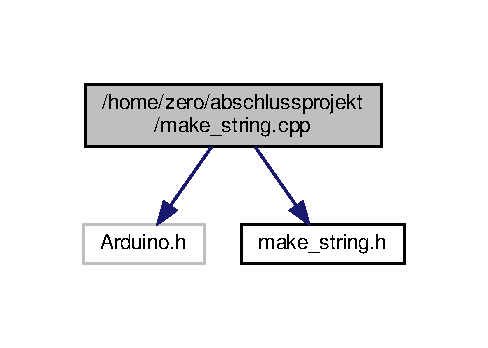
\includegraphics[width=234pt]{make__string_8cpp__incl}
\end{center}
\end{figure}
\subsection*{Funktionen}
\begin{DoxyCompactItemize}
\item 
String \hyperlink{make__string_8cpp_a19ab0f1c20c9a665b3a65c5422e817a9}{make\+\_\+string} (String s)
\end{DoxyCompactItemize}


\subsection{Dokumentation der Funktionen}
\mbox{\Hypertarget{make__string_8cpp_a19ab0f1c20c9a665b3a65c5422e817a9}\label{make__string_8cpp_a19ab0f1c20c9a665b3a65c5422e817a9}} 
\index{make\+\_\+string.\+cpp@{make\+\_\+string.\+cpp}!make\+\_\+string@{make\+\_\+string}}
\index{make\+\_\+string@{make\+\_\+string}!make\+\_\+string.\+cpp@{make\+\_\+string.\+cpp}}
\subsubsection{\texorpdfstring{make\+\_\+string()}{make\_string()}}
{\footnotesize\ttfamily String make\+\_\+string (\begin{DoxyParamCaption}\item[{String}]{s }\end{DoxyParamCaption})}



Definiert in Zeile 5 der Datei make\+\_\+string.\+cpp.


\hypertarget{make__string_8h}{}\section{/home/zero/abschlussprojekt/make\+\_\+string.h-\/\+Dateireferenz}
\label{make__string_8h}\index{/home/zero/abschlussprojekt/make\+\_\+string.\+h@{/home/zero/abschlussprojekt/make\+\_\+string.\+h}}
Dieser Graph zeigt, welche Datei direkt oder indirekt diese Datei enthält\+:
\nopagebreak
\begin{figure}[H]
\begin{center}
\leavevmode
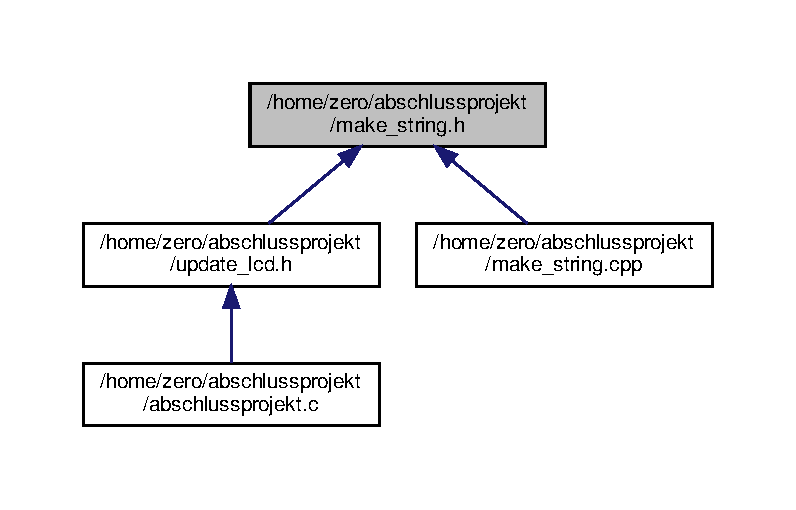
\includegraphics[width=350pt]{make__string_8h__dep__incl}
\end{center}
\end{figure}
\subsection*{Funktionen}
\begin{DoxyCompactItemize}
\item 
String \hyperlink{make__string_8h_a19ab0f1c20c9a665b3a65c5422e817a9}{make\+\_\+string} (String s)
\end{DoxyCompactItemize}


\subsection{Dokumentation der Funktionen}
\mbox{\Hypertarget{make__string_8h_a19ab0f1c20c9a665b3a65c5422e817a9}\label{make__string_8h_a19ab0f1c20c9a665b3a65c5422e817a9}} 
\index{make\+\_\+string.\+h@{make\+\_\+string.\+h}!make\+\_\+string@{make\+\_\+string}}
\index{make\+\_\+string@{make\+\_\+string}!make\+\_\+string.\+h@{make\+\_\+string.\+h}}
\subsubsection{\texorpdfstring{make\+\_\+string()}{make\_string()}}
{\footnotesize\ttfamily String make\+\_\+string (\begin{DoxyParamCaption}\item[{String}]{s }\end{DoxyParamCaption})}



Definiert in Zeile 5 der Datei make\+\_\+string.\+cpp.


\hypertarget{makros_8h}{}\section{/home/zero/abschlussprojekt/makros.h-\/\+Dateireferenz}
\label{makros_8h}\index{/home/zero/abschlussprojekt/makros.\+h@{/home/zero/abschlussprojekt/makros.\+h}}
{\ttfamily \#include $<$Arduino.\+h$>$}\newline
Include-\/\+Abhängigkeitsdiagramm für makros.\+h\+:
\nopagebreak
\begin{figure}[H]
\begin{center}
\leavevmode
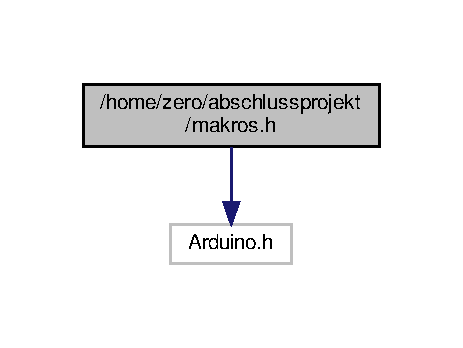
\includegraphics[width=222pt]{makros_8h__incl}
\end{center}
\end{figure}
Dieser Graph zeigt, welche Datei direkt oder indirekt diese Datei enthält\+:
\nopagebreak
\begin{figure}[H]
\begin{center}
\leavevmode
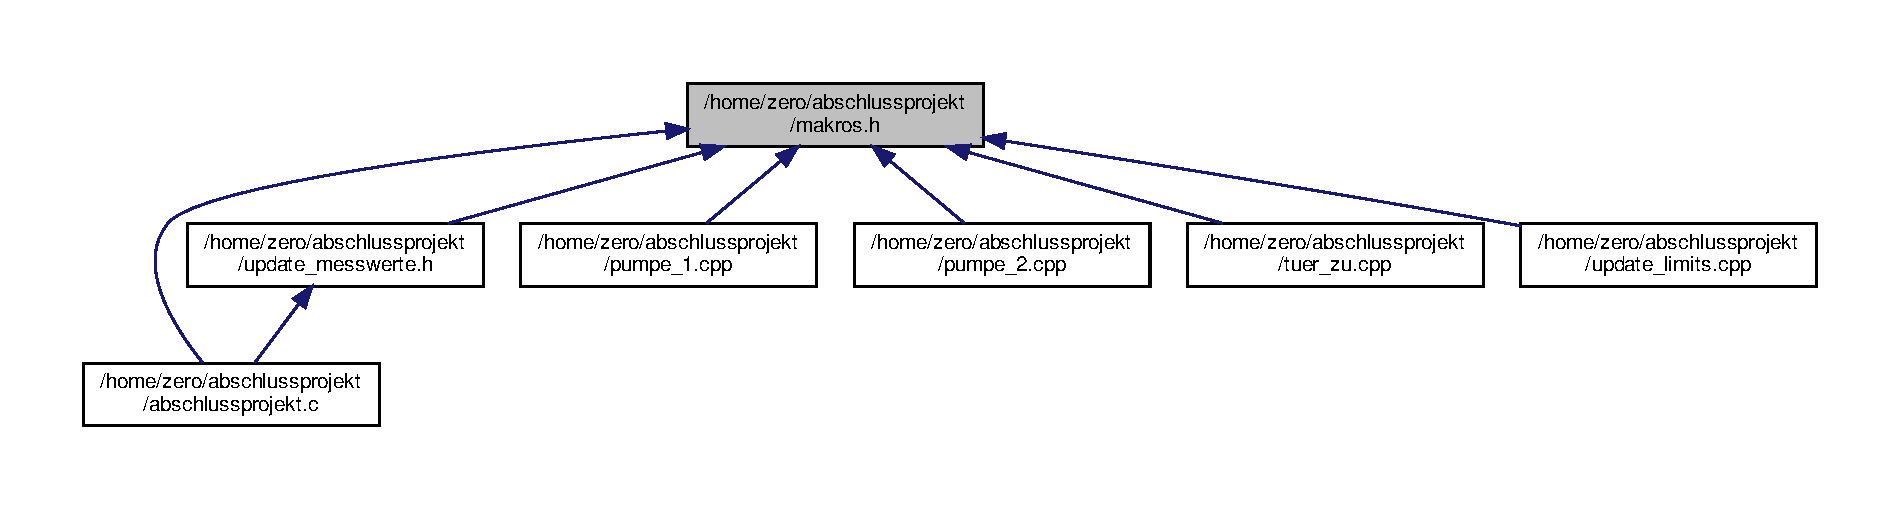
\includegraphics[width=350pt]{makros_8h__dep__incl}
\end{center}
\end{figure}
\subsection*{Makrodefinitionen}
\begin{DoxyCompactItemize}
\item 
\#define \hyperlink{makros_8h_a2c509dba12bba99883a5be9341b7a0c5}{D\+H\+T\+T\+Y\+PE}~D\+H\+T22
\item 
\#define \hyperlink{makros_8h_a3edd9adbe80cfa6949a85935a79275d7}{T\+A\+S\+T\+E\+R\+\_\+\+D\+I\+S\+P\+L\+AY}~2
\item 
\#define \hyperlink{makros_8h_ae5585e7e3d65edaff2d78517eb4f759d}{R\+E\+L\+A\+I\+S\+\_\+\+P\+U\+M\+P\+E\+\_\+\+O\+B\+EN}~4
\item 
\#define \hyperlink{makros_8h_a2f5672d9a8ae3f2d5a148adbb8143c68}{R\+E\+L\+A\+I\+S\+\_\+\+P\+U\+M\+P\+E\+\_\+\+U\+N\+T\+EN}~5
\item 
\#define \hyperlink{makros_8h_a30d6fbf03c0e3ae5cf71977fe9dfa1d5}{R\+E\+L\+A\+I\+S\+\_\+\+L\+U\+E\+F\+T\+ER}~6
\item 
\#define \hyperlink{makros_8h_a5316bb60c0bf0c793c28ba8815caa69b}{R\+E\+L\+A\+I\+S\+\_\+\+U\+V\+\_\+\+L\+ED}~7
\item 
\#define \hyperlink{makros_8h_a2fc336b6f27547c3b2f8e501806d95e2}{R\+E\+L\+A\+I\+S\+\_\+\+H\+E\+I\+Z\+U\+NG}~8
\item 
\#define \hyperlink{makros_8h_a9894c05769fdf48b3506408030591a65}{T\+E\+M\+P\+E\+R\+A\+T\+U\+R\+S\+E\+N\+S\+O\+R\+\_\+\+L\+U\+E\+F\+T\+ER}~9
\item 
\#define \hyperlink{makros_8h_abd1dbbe0460847d74097b3fbb78d9457}{H\+E\+L\+L\+I\+G\+K\+E\+I\+T\+S\+S\+E\+N\+S\+OR}~10
\item 
\#define \hyperlink{makros_8h_aa5c8a88c5a3dde80789f0b329b877a6f}{R\+E\+E\+D\+K\+O\+N\+T\+A\+KT}~11
\item 
\#define \hyperlink{makros_8h_a217a0b1523cc63a0e9618b0b9bcc3944}{E\+R\+D\+F\+E\+U\+C\+H\+T\+E\+S\+E\+N\+S\+O\+R\+\_\+1}~A0
\item 
\#define \hyperlink{makros_8h_ab35f6b04d1873122637b48a378828072}{E\+R\+D\+F\+E\+U\+C\+H\+T\+E\+S\+E\+N\+S\+O\+R\+\_\+2}~A1
\item 
\#define \hyperlink{makros_8h_a2cfb9232ef93fe3dbe489ea0ed78ab5c}{L\+I\+M\+I\+T\+\_\+\+E\+R\+D\+F\+E\+U\+C\+H\+T\+E\+\_\+1}~A2
\item 
\#define \hyperlink{makros_8h_a06863b5c4eac468b904afed8c6c36440}{L\+I\+M\+I\+T\+\_\+\+E\+R\+D\+F\+E\+U\+C\+H\+T\+E\+\_\+2}~A3
\item 
\#define \hyperlink{makros_8h_ae07fe35374a1fd6e6d921bd39ba73b99}{L\+I\+M\+I\+T\+\_\+\+T\+E\+M\+P\+E\+R\+A\+T\+UR}~A6
\item 
\#define \hyperlink{makros_8h_a392b9a22bb52d29603ffb57ab4255e86}{L\+I\+M\+I\+T\+\_\+\+L\+U\+E\+F\+T\+ER}~A5
\item 
\#define \hyperlink{makros_8h_acd99f73b20037e5fcba7a4a031e0f320}{zustand\+\_\+warten\+\_\+zu\+\_\+trocken}~0
\item 
\#define \hyperlink{makros_8h_a451a24326bd3759cea1cbd0da8d4bb12}{zustand\+\_\+pumpt}~1
\item 
\#define \hyperlink{makros_8h_a15e9e3e52a86bfb566502710f2453c20}{zustand\+\_\+warten\+\_\+durchfeuchtung}~2
\end{DoxyCompactItemize}


\subsection{Makro-\/\+Dokumentation}
\mbox{\Hypertarget{makros_8h_a2c509dba12bba99883a5be9341b7a0c5}\label{makros_8h_a2c509dba12bba99883a5be9341b7a0c5}} 
\index{makros.\+h@{makros.\+h}!D\+H\+T\+T\+Y\+PE@{D\+H\+T\+T\+Y\+PE}}
\index{D\+H\+T\+T\+Y\+PE@{D\+H\+T\+T\+Y\+PE}!makros.\+h@{makros.\+h}}
\subsubsection{\texorpdfstring{D\+H\+T\+T\+Y\+PE}{DHTTYPE}}
{\footnotesize\ttfamily \#define D\+H\+T\+T\+Y\+PE~D\+H\+T22}



Definiert in Zeile 8 der Datei makros.\+h.

\mbox{\Hypertarget{makros_8h_a217a0b1523cc63a0e9618b0b9bcc3944}\label{makros_8h_a217a0b1523cc63a0e9618b0b9bcc3944}} 
\index{makros.\+h@{makros.\+h}!E\+R\+D\+F\+E\+U\+C\+H\+T\+E\+S\+E\+N\+S\+O\+R\+\_\+1@{E\+R\+D\+F\+E\+U\+C\+H\+T\+E\+S\+E\+N\+S\+O\+R\+\_\+1}}
\index{E\+R\+D\+F\+E\+U\+C\+H\+T\+E\+S\+E\+N\+S\+O\+R\+\_\+1@{E\+R\+D\+F\+E\+U\+C\+H\+T\+E\+S\+E\+N\+S\+O\+R\+\_\+1}!makros.\+h@{makros.\+h}}
\subsubsection{\texorpdfstring{E\+R\+D\+F\+E\+U\+C\+H\+T\+E\+S\+E\+N\+S\+O\+R\+\_\+1}{ERDFEUCHTESENSOR\_1}}
{\footnotesize\ttfamily \#define E\+R\+D\+F\+E\+U\+C\+H\+T\+E\+S\+E\+N\+S\+O\+R\+\_\+1~A0}



Definiert in Zeile 20 der Datei makros.\+h.

\mbox{\Hypertarget{makros_8h_ab35f6b04d1873122637b48a378828072}\label{makros_8h_ab35f6b04d1873122637b48a378828072}} 
\index{makros.\+h@{makros.\+h}!E\+R\+D\+F\+E\+U\+C\+H\+T\+E\+S\+E\+N\+S\+O\+R\+\_\+2@{E\+R\+D\+F\+E\+U\+C\+H\+T\+E\+S\+E\+N\+S\+O\+R\+\_\+2}}
\index{E\+R\+D\+F\+E\+U\+C\+H\+T\+E\+S\+E\+N\+S\+O\+R\+\_\+2@{E\+R\+D\+F\+E\+U\+C\+H\+T\+E\+S\+E\+N\+S\+O\+R\+\_\+2}!makros.\+h@{makros.\+h}}
\subsubsection{\texorpdfstring{E\+R\+D\+F\+E\+U\+C\+H\+T\+E\+S\+E\+N\+S\+O\+R\+\_\+2}{ERDFEUCHTESENSOR\_2}}
{\footnotesize\ttfamily \#define E\+R\+D\+F\+E\+U\+C\+H\+T\+E\+S\+E\+N\+S\+O\+R\+\_\+2~A1}



Definiert in Zeile 21 der Datei makros.\+h.

\mbox{\Hypertarget{makros_8h_abd1dbbe0460847d74097b3fbb78d9457}\label{makros_8h_abd1dbbe0460847d74097b3fbb78d9457}} 
\index{makros.\+h@{makros.\+h}!H\+E\+L\+L\+I\+G\+K\+E\+I\+T\+S\+S\+E\+N\+S\+OR@{H\+E\+L\+L\+I\+G\+K\+E\+I\+T\+S\+S\+E\+N\+S\+OR}}
\index{H\+E\+L\+L\+I\+G\+K\+E\+I\+T\+S\+S\+E\+N\+S\+OR@{H\+E\+L\+L\+I\+G\+K\+E\+I\+T\+S\+S\+E\+N\+S\+OR}!makros.\+h@{makros.\+h}}
\subsubsection{\texorpdfstring{H\+E\+L\+L\+I\+G\+K\+E\+I\+T\+S\+S\+E\+N\+S\+OR}{HELLIGKEITSSENSOR}}
{\footnotesize\ttfamily \#define H\+E\+L\+L\+I\+G\+K\+E\+I\+T\+S\+S\+E\+N\+S\+OR~10}



Definiert in Zeile 16 der Datei makros.\+h.

\mbox{\Hypertarget{makros_8h_a2cfb9232ef93fe3dbe489ea0ed78ab5c}\label{makros_8h_a2cfb9232ef93fe3dbe489ea0ed78ab5c}} 
\index{makros.\+h@{makros.\+h}!L\+I\+M\+I\+T\+\_\+\+E\+R\+D\+F\+E\+U\+C\+H\+T\+E\+\_\+1@{L\+I\+M\+I\+T\+\_\+\+E\+R\+D\+F\+E\+U\+C\+H\+T\+E\+\_\+1}}
\index{L\+I\+M\+I\+T\+\_\+\+E\+R\+D\+F\+E\+U\+C\+H\+T\+E\+\_\+1@{L\+I\+M\+I\+T\+\_\+\+E\+R\+D\+F\+E\+U\+C\+H\+T\+E\+\_\+1}!makros.\+h@{makros.\+h}}
\subsubsection{\texorpdfstring{L\+I\+M\+I\+T\+\_\+\+E\+R\+D\+F\+E\+U\+C\+H\+T\+E\+\_\+1}{LIMIT\_ERDFEUCHTE\_1}}
{\footnotesize\ttfamily \#define L\+I\+M\+I\+T\+\_\+\+E\+R\+D\+F\+E\+U\+C\+H\+T\+E\+\_\+1~A2}



Definiert in Zeile 22 der Datei makros.\+h.

\mbox{\Hypertarget{makros_8h_a06863b5c4eac468b904afed8c6c36440}\label{makros_8h_a06863b5c4eac468b904afed8c6c36440}} 
\index{makros.\+h@{makros.\+h}!L\+I\+M\+I\+T\+\_\+\+E\+R\+D\+F\+E\+U\+C\+H\+T\+E\+\_\+2@{L\+I\+M\+I\+T\+\_\+\+E\+R\+D\+F\+E\+U\+C\+H\+T\+E\+\_\+2}}
\index{L\+I\+M\+I\+T\+\_\+\+E\+R\+D\+F\+E\+U\+C\+H\+T\+E\+\_\+2@{L\+I\+M\+I\+T\+\_\+\+E\+R\+D\+F\+E\+U\+C\+H\+T\+E\+\_\+2}!makros.\+h@{makros.\+h}}
\subsubsection{\texorpdfstring{L\+I\+M\+I\+T\+\_\+\+E\+R\+D\+F\+E\+U\+C\+H\+T\+E\+\_\+2}{LIMIT\_ERDFEUCHTE\_2}}
{\footnotesize\ttfamily \#define L\+I\+M\+I\+T\+\_\+\+E\+R\+D\+F\+E\+U\+C\+H\+T\+E\+\_\+2~A3}



Definiert in Zeile 23 der Datei makros.\+h.

\mbox{\Hypertarget{makros_8h_a392b9a22bb52d29603ffb57ab4255e86}\label{makros_8h_a392b9a22bb52d29603ffb57ab4255e86}} 
\index{makros.\+h@{makros.\+h}!L\+I\+M\+I\+T\+\_\+\+L\+U\+E\+F\+T\+ER@{L\+I\+M\+I\+T\+\_\+\+L\+U\+E\+F\+T\+ER}}
\index{L\+I\+M\+I\+T\+\_\+\+L\+U\+E\+F\+T\+ER@{L\+I\+M\+I\+T\+\_\+\+L\+U\+E\+F\+T\+ER}!makros.\+h@{makros.\+h}}
\subsubsection{\texorpdfstring{L\+I\+M\+I\+T\+\_\+\+L\+U\+E\+F\+T\+ER}{LIMIT\_LUEFTER}}
{\footnotesize\ttfamily \#define L\+I\+M\+I\+T\+\_\+\+L\+U\+E\+F\+T\+ER~A5}



Definiert in Zeile 25 der Datei makros.\+h.

\mbox{\Hypertarget{makros_8h_ae07fe35374a1fd6e6d921bd39ba73b99}\label{makros_8h_ae07fe35374a1fd6e6d921bd39ba73b99}} 
\index{makros.\+h@{makros.\+h}!L\+I\+M\+I\+T\+\_\+\+T\+E\+M\+P\+E\+R\+A\+T\+UR@{L\+I\+M\+I\+T\+\_\+\+T\+E\+M\+P\+E\+R\+A\+T\+UR}}
\index{L\+I\+M\+I\+T\+\_\+\+T\+E\+M\+P\+E\+R\+A\+T\+UR@{L\+I\+M\+I\+T\+\_\+\+T\+E\+M\+P\+E\+R\+A\+T\+UR}!makros.\+h@{makros.\+h}}
\subsubsection{\texorpdfstring{L\+I\+M\+I\+T\+\_\+\+T\+E\+M\+P\+E\+R\+A\+T\+UR}{LIMIT\_TEMPERATUR}}
{\footnotesize\ttfamily \#define L\+I\+M\+I\+T\+\_\+\+T\+E\+M\+P\+E\+R\+A\+T\+UR~A6}



Definiert in Zeile 24 der Datei makros.\+h.

\mbox{\Hypertarget{makros_8h_aa5c8a88c5a3dde80789f0b329b877a6f}\label{makros_8h_aa5c8a88c5a3dde80789f0b329b877a6f}} 
\index{makros.\+h@{makros.\+h}!R\+E\+E\+D\+K\+O\+N\+T\+A\+KT@{R\+E\+E\+D\+K\+O\+N\+T\+A\+KT}}
\index{R\+E\+E\+D\+K\+O\+N\+T\+A\+KT@{R\+E\+E\+D\+K\+O\+N\+T\+A\+KT}!makros.\+h@{makros.\+h}}
\subsubsection{\texorpdfstring{R\+E\+E\+D\+K\+O\+N\+T\+A\+KT}{REEDKONTAKT}}
{\footnotesize\ttfamily \#define R\+E\+E\+D\+K\+O\+N\+T\+A\+KT~11}



Definiert in Zeile 17 der Datei makros.\+h.

\mbox{\Hypertarget{makros_8h_a2fc336b6f27547c3b2f8e501806d95e2}\label{makros_8h_a2fc336b6f27547c3b2f8e501806d95e2}} 
\index{makros.\+h@{makros.\+h}!R\+E\+L\+A\+I\+S\+\_\+\+H\+E\+I\+Z\+U\+NG@{R\+E\+L\+A\+I\+S\+\_\+\+H\+E\+I\+Z\+U\+NG}}
\index{R\+E\+L\+A\+I\+S\+\_\+\+H\+E\+I\+Z\+U\+NG@{R\+E\+L\+A\+I\+S\+\_\+\+H\+E\+I\+Z\+U\+NG}!makros.\+h@{makros.\+h}}
\subsubsection{\texorpdfstring{R\+E\+L\+A\+I\+S\+\_\+\+H\+E\+I\+Z\+U\+NG}{RELAIS\_HEIZUNG}}
{\footnotesize\ttfamily \#define R\+E\+L\+A\+I\+S\+\_\+\+H\+E\+I\+Z\+U\+NG~8}



Definiert in Zeile 14 der Datei makros.\+h.

\mbox{\Hypertarget{makros_8h_a30d6fbf03c0e3ae5cf71977fe9dfa1d5}\label{makros_8h_a30d6fbf03c0e3ae5cf71977fe9dfa1d5}} 
\index{makros.\+h@{makros.\+h}!R\+E\+L\+A\+I\+S\+\_\+\+L\+U\+E\+F\+T\+ER@{R\+E\+L\+A\+I\+S\+\_\+\+L\+U\+E\+F\+T\+ER}}
\index{R\+E\+L\+A\+I\+S\+\_\+\+L\+U\+E\+F\+T\+ER@{R\+E\+L\+A\+I\+S\+\_\+\+L\+U\+E\+F\+T\+ER}!makros.\+h@{makros.\+h}}
\subsubsection{\texorpdfstring{R\+E\+L\+A\+I\+S\+\_\+\+L\+U\+E\+F\+T\+ER}{RELAIS\_LUEFTER}}
{\footnotesize\ttfamily \#define R\+E\+L\+A\+I\+S\+\_\+\+L\+U\+E\+F\+T\+ER~6}



Definiert in Zeile 12 der Datei makros.\+h.

\mbox{\Hypertarget{makros_8h_ae5585e7e3d65edaff2d78517eb4f759d}\label{makros_8h_ae5585e7e3d65edaff2d78517eb4f759d}} 
\index{makros.\+h@{makros.\+h}!R\+E\+L\+A\+I\+S\+\_\+\+P\+U\+M\+P\+E\+\_\+\+O\+B\+EN@{R\+E\+L\+A\+I\+S\+\_\+\+P\+U\+M\+P\+E\+\_\+\+O\+B\+EN}}
\index{R\+E\+L\+A\+I\+S\+\_\+\+P\+U\+M\+P\+E\+\_\+\+O\+B\+EN@{R\+E\+L\+A\+I\+S\+\_\+\+P\+U\+M\+P\+E\+\_\+\+O\+B\+EN}!makros.\+h@{makros.\+h}}
\subsubsection{\texorpdfstring{R\+E\+L\+A\+I\+S\+\_\+\+P\+U\+M\+P\+E\+\_\+\+O\+B\+EN}{RELAIS\_PUMPE\_OBEN}}
{\footnotesize\ttfamily \#define R\+E\+L\+A\+I\+S\+\_\+\+P\+U\+M\+P\+E\+\_\+\+O\+B\+EN~4}



Definiert in Zeile 10 der Datei makros.\+h.

\mbox{\Hypertarget{makros_8h_a2f5672d9a8ae3f2d5a148adbb8143c68}\label{makros_8h_a2f5672d9a8ae3f2d5a148adbb8143c68}} 
\index{makros.\+h@{makros.\+h}!R\+E\+L\+A\+I\+S\+\_\+\+P\+U\+M\+P\+E\+\_\+\+U\+N\+T\+EN@{R\+E\+L\+A\+I\+S\+\_\+\+P\+U\+M\+P\+E\+\_\+\+U\+N\+T\+EN}}
\index{R\+E\+L\+A\+I\+S\+\_\+\+P\+U\+M\+P\+E\+\_\+\+U\+N\+T\+EN@{R\+E\+L\+A\+I\+S\+\_\+\+P\+U\+M\+P\+E\+\_\+\+U\+N\+T\+EN}!makros.\+h@{makros.\+h}}
\subsubsection{\texorpdfstring{R\+E\+L\+A\+I\+S\+\_\+\+P\+U\+M\+P\+E\+\_\+\+U\+N\+T\+EN}{RELAIS\_PUMPE\_UNTEN}}
{\footnotesize\ttfamily \#define R\+E\+L\+A\+I\+S\+\_\+\+P\+U\+M\+P\+E\+\_\+\+U\+N\+T\+EN~5}



Definiert in Zeile 11 der Datei makros.\+h.

\mbox{\Hypertarget{makros_8h_a5316bb60c0bf0c793c28ba8815caa69b}\label{makros_8h_a5316bb60c0bf0c793c28ba8815caa69b}} 
\index{makros.\+h@{makros.\+h}!R\+E\+L\+A\+I\+S\+\_\+\+U\+V\+\_\+\+L\+ED@{R\+E\+L\+A\+I\+S\+\_\+\+U\+V\+\_\+\+L\+ED}}
\index{R\+E\+L\+A\+I\+S\+\_\+\+U\+V\+\_\+\+L\+ED@{R\+E\+L\+A\+I\+S\+\_\+\+U\+V\+\_\+\+L\+ED}!makros.\+h@{makros.\+h}}
\subsubsection{\texorpdfstring{R\+E\+L\+A\+I\+S\+\_\+\+U\+V\+\_\+\+L\+ED}{RELAIS\_UV\_LED}}
{\footnotesize\ttfamily \#define R\+E\+L\+A\+I\+S\+\_\+\+U\+V\+\_\+\+L\+ED~7}



Definiert in Zeile 13 der Datei makros.\+h.

\mbox{\Hypertarget{makros_8h_a3edd9adbe80cfa6949a85935a79275d7}\label{makros_8h_a3edd9adbe80cfa6949a85935a79275d7}} 
\index{makros.\+h@{makros.\+h}!T\+A\+S\+T\+E\+R\+\_\+\+D\+I\+S\+P\+L\+AY@{T\+A\+S\+T\+E\+R\+\_\+\+D\+I\+S\+P\+L\+AY}}
\index{T\+A\+S\+T\+E\+R\+\_\+\+D\+I\+S\+P\+L\+AY@{T\+A\+S\+T\+E\+R\+\_\+\+D\+I\+S\+P\+L\+AY}!makros.\+h@{makros.\+h}}
\subsubsection{\texorpdfstring{T\+A\+S\+T\+E\+R\+\_\+\+D\+I\+S\+P\+L\+AY}{TASTER\_DISPLAY}}
{\footnotesize\ttfamily \#define T\+A\+S\+T\+E\+R\+\_\+\+D\+I\+S\+P\+L\+AY~2}



Definiert in Zeile 9 der Datei makros.\+h.

\mbox{\Hypertarget{makros_8h_a9894c05769fdf48b3506408030591a65}\label{makros_8h_a9894c05769fdf48b3506408030591a65}} 
\index{makros.\+h@{makros.\+h}!T\+E\+M\+P\+E\+R\+A\+T\+U\+R\+S\+E\+N\+S\+O\+R\+\_\+\+L\+U\+E\+F\+T\+ER@{T\+E\+M\+P\+E\+R\+A\+T\+U\+R\+S\+E\+N\+S\+O\+R\+\_\+\+L\+U\+E\+F\+T\+ER}}
\index{T\+E\+M\+P\+E\+R\+A\+T\+U\+R\+S\+E\+N\+S\+O\+R\+\_\+\+L\+U\+E\+F\+T\+ER@{T\+E\+M\+P\+E\+R\+A\+T\+U\+R\+S\+E\+N\+S\+O\+R\+\_\+\+L\+U\+E\+F\+T\+ER}!makros.\+h@{makros.\+h}}
\subsubsection{\texorpdfstring{T\+E\+M\+P\+E\+R\+A\+T\+U\+R\+S\+E\+N\+S\+O\+R\+\_\+\+L\+U\+E\+F\+T\+ER}{TEMPERATURSENSOR\_LUEFTER}}
{\footnotesize\ttfamily \#define T\+E\+M\+P\+E\+R\+A\+T\+U\+R\+S\+E\+N\+S\+O\+R\+\_\+\+L\+U\+E\+F\+T\+ER~9}



Definiert in Zeile 15 der Datei makros.\+h.

\mbox{\Hypertarget{makros_8h_a451a24326bd3759cea1cbd0da8d4bb12}\label{makros_8h_a451a24326bd3759cea1cbd0da8d4bb12}} 
\index{makros.\+h@{makros.\+h}!zustand\+\_\+pumpt@{zustand\+\_\+pumpt}}
\index{zustand\+\_\+pumpt@{zustand\+\_\+pumpt}!makros.\+h@{makros.\+h}}
\subsubsection{\texorpdfstring{zustand\+\_\+pumpt}{zustand\_pumpt}}
{\footnotesize\ttfamily \#define zustand\+\_\+pumpt~1}



Definiert in Zeile 29 der Datei makros.\+h.

\mbox{\Hypertarget{makros_8h_a15e9e3e52a86bfb566502710f2453c20}\label{makros_8h_a15e9e3e52a86bfb566502710f2453c20}} 
\index{makros.\+h@{makros.\+h}!zustand\+\_\+warten\+\_\+durchfeuchtung@{zustand\+\_\+warten\+\_\+durchfeuchtung}}
\index{zustand\+\_\+warten\+\_\+durchfeuchtung@{zustand\+\_\+warten\+\_\+durchfeuchtung}!makros.\+h@{makros.\+h}}
\subsubsection{\texorpdfstring{zustand\+\_\+warten\+\_\+durchfeuchtung}{zustand\_warten\_durchfeuchtung}}
{\footnotesize\ttfamily \#define zustand\+\_\+warten\+\_\+durchfeuchtung~2}



Definiert in Zeile 30 der Datei makros.\+h.

\mbox{\Hypertarget{makros_8h_acd99f73b20037e5fcba7a4a031e0f320}\label{makros_8h_acd99f73b20037e5fcba7a4a031e0f320}} 
\index{makros.\+h@{makros.\+h}!zustand\+\_\+warten\+\_\+zu\+\_\+trocken@{zustand\+\_\+warten\+\_\+zu\+\_\+trocken}}
\index{zustand\+\_\+warten\+\_\+zu\+\_\+trocken@{zustand\+\_\+warten\+\_\+zu\+\_\+trocken}!makros.\+h@{makros.\+h}}
\subsubsection{\texorpdfstring{zustand\+\_\+warten\+\_\+zu\+\_\+trocken}{zustand\_warten\_zu\_trocken}}
{\footnotesize\ttfamily \#define zustand\+\_\+warten\+\_\+zu\+\_\+trocken~0}



Definiert in Zeile 28 der Datei makros.\+h.


\hypertarget{pumpe__1_8cpp}{}\section{/home/zero/abschlussprojekt/pumpe\+\_\+1.cpp-\/\+Dateireferenz}
\label{pumpe__1_8cpp}\index{/home/zero/abschlussprojekt/pumpe\+\_\+1.\+cpp@{/home/zero/abschlussprojekt/pumpe\+\_\+1.\+cpp}}
{\ttfamily \#include $<$Arduino.\+h$>$}\newline
{\ttfamily \#include \char`\"{}makros.\+h\char`\"{}}\newline
{\ttfamily \#include \char`\"{}tuer\+\_\+zu.\+h\char`\"{}}\newline
{\ttfamily \#include \char`\"{}pumpe\+\_\+1.\+h\char`\"{}}\newline
Include-\/\+Abhängigkeitsdiagramm für pumpe\+\_\+1.\+cpp\+:
\nopagebreak
\begin{figure}[H]
\begin{center}
\leavevmode
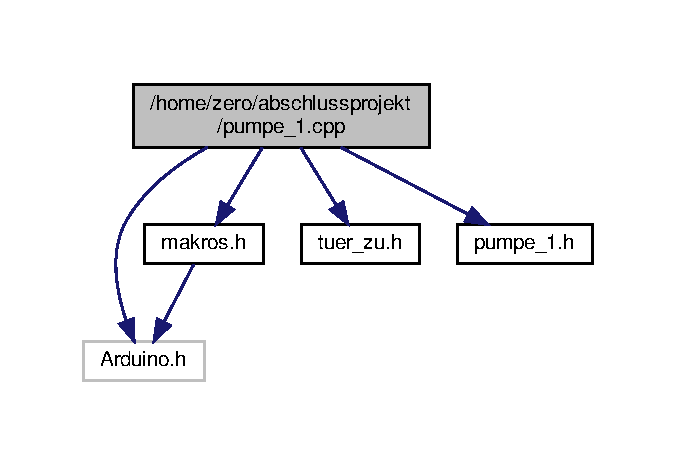
\includegraphics[width=325pt]{pumpe__1_8cpp__incl}
\end{center}
\end{figure}
\subsection*{Funktionen}
\begin{DoxyCompactItemize}
\item 
void \hyperlink{pumpe__1_8cpp_ab395b141ee439daa2552b2aee993de59}{pumpen\+\_\+1} ()
\begin{DoxyCompactList}\small\item\em Zustandsautomat Pumpe 1 ///. \end{DoxyCompactList}\end{DoxyCompactItemize}
\subsection*{Variablen}
\begin{DoxyCompactItemize}
\item 
int \hyperlink{pumpe__1_8cpp_afa416e7460cf043207be351d750b97fe}{hum\+\_\+erde\+\_\+1\+\_\+adc}
\item 
int \hyperlink{pumpe__1_8cpp_abb1c509cfb119e70585771234accdc4c}{limit\+\_\+feuchte\+\_\+1\+\_\+adc}
\item 
unsigned long \hyperlink{pumpe__1_8cpp_abb7944bc8f9499e8ee84d361d823f122}{t0\+\_\+pumpe\+\_\+1}
\item 
unsigned long \hyperlink{pumpe__1_8cpp_ad2fcb732158343baf6f03db3f44377d0}{dt\+\_\+pumpendauer\+\_\+1\+\_\+ms} = 5000
\item 
unsigned long \hyperlink{pumpe__1_8cpp_a562f2a69077e9416bef8bcb843261334}{t0\+\_\+durchfeuchtung\+\_\+1}
\item 
unsigned long \hyperlink{pumpe__1_8cpp_a8dcdc9f5bd8d9fd59fdf7a54869ebd81}{dt\+\_\+warten\+\_\+durchfeuchtung\+\_\+1\+\_\+ms} = 10000
\item 
int \hyperlink{pumpe__1_8cpp_a312a74000d8f9d74536e66d0a5e7bfc4}{zustand\+\_\+1} = \hyperlink{makros_8h_acd99f73b20037e5fcba7a4a031e0f320}{zustand\+\_\+warten\+\_\+zu\+\_\+trocken}
\end{DoxyCompactItemize}


\subsection{Dokumentation der Funktionen}
\mbox{\Hypertarget{pumpe__1_8cpp_ab395b141ee439daa2552b2aee993de59}\label{pumpe__1_8cpp_ab395b141ee439daa2552b2aee993de59}} 
\index{pumpe\+\_\+1.\+cpp@{pumpe\+\_\+1.\+cpp}!pumpen\+\_\+1@{pumpen\+\_\+1}}
\index{pumpen\+\_\+1@{pumpen\+\_\+1}!pumpe\+\_\+1.\+cpp@{pumpe\+\_\+1.\+cpp}}
\subsubsection{\texorpdfstring{pumpen\+\_\+1()}{pumpen\_1()}}
{\footnotesize\ttfamily void pumpen\+\_\+1 (\begin{DoxyParamCaption}\item[{void}]{ }\end{DoxyParamCaption})}



Zustandsautomat Pumpe 1 ///. 



Definiert in Zeile 16 der Datei pumpe\+\_\+1.\+cpp.



\subsection{Variablen-\/\+Dokumentation}
\mbox{\Hypertarget{pumpe__1_8cpp_ad2fcb732158343baf6f03db3f44377d0}\label{pumpe__1_8cpp_ad2fcb732158343baf6f03db3f44377d0}} 
\index{pumpe\+\_\+1.\+cpp@{pumpe\+\_\+1.\+cpp}!dt\+\_\+pumpendauer\+\_\+1\+\_\+ms@{dt\+\_\+pumpendauer\+\_\+1\+\_\+ms}}
\index{dt\+\_\+pumpendauer\+\_\+1\+\_\+ms@{dt\+\_\+pumpendauer\+\_\+1\+\_\+ms}!pumpe\+\_\+1.\+cpp@{pumpe\+\_\+1.\+cpp}}
\subsubsection{\texorpdfstring{dt\+\_\+pumpendauer\+\_\+1\+\_\+ms}{dt\_pumpendauer\_1\_ms}}
{\footnotesize\ttfamily unsigned long dt\+\_\+pumpendauer\+\_\+1\+\_\+ms = 5000}



Definiert in Zeile 10 der Datei pumpe\+\_\+1.\+cpp.

\mbox{\Hypertarget{pumpe__1_8cpp_a8dcdc9f5bd8d9fd59fdf7a54869ebd81}\label{pumpe__1_8cpp_a8dcdc9f5bd8d9fd59fdf7a54869ebd81}} 
\index{pumpe\+\_\+1.\+cpp@{pumpe\+\_\+1.\+cpp}!dt\+\_\+warten\+\_\+durchfeuchtung\+\_\+1\+\_\+ms@{dt\+\_\+warten\+\_\+durchfeuchtung\+\_\+1\+\_\+ms}}
\index{dt\+\_\+warten\+\_\+durchfeuchtung\+\_\+1\+\_\+ms@{dt\+\_\+warten\+\_\+durchfeuchtung\+\_\+1\+\_\+ms}!pumpe\+\_\+1.\+cpp@{pumpe\+\_\+1.\+cpp}}
\subsubsection{\texorpdfstring{dt\+\_\+warten\+\_\+durchfeuchtung\+\_\+1\+\_\+ms}{dt\_warten\_durchfeuchtung\_1\_ms}}
{\footnotesize\ttfamily unsigned long dt\+\_\+warten\+\_\+durchfeuchtung\+\_\+1\+\_\+ms = 10000}



Definiert in Zeile 12 der Datei pumpe\+\_\+1.\+cpp.

\mbox{\Hypertarget{pumpe__1_8cpp_afa416e7460cf043207be351d750b97fe}\label{pumpe__1_8cpp_afa416e7460cf043207be351d750b97fe}} 
\index{pumpe\+\_\+1.\+cpp@{pumpe\+\_\+1.\+cpp}!hum\+\_\+erde\+\_\+1\+\_\+adc@{hum\+\_\+erde\+\_\+1\+\_\+adc}}
\index{hum\+\_\+erde\+\_\+1\+\_\+adc@{hum\+\_\+erde\+\_\+1\+\_\+adc}!pumpe\+\_\+1.\+cpp@{pumpe\+\_\+1.\+cpp}}
\subsubsection{\texorpdfstring{hum\+\_\+erde\+\_\+1\+\_\+adc}{hum\_erde\_1\_adc}}
{\footnotesize\ttfamily int hum\+\_\+erde\+\_\+1\+\_\+adc}



Definiert in Zeile 46 der Datei abschlussprojekt.\+c.

\mbox{\Hypertarget{pumpe__1_8cpp_abb1c509cfb119e70585771234accdc4c}\label{pumpe__1_8cpp_abb1c509cfb119e70585771234accdc4c}} 
\index{pumpe\+\_\+1.\+cpp@{pumpe\+\_\+1.\+cpp}!limit\+\_\+feuchte\+\_\+1\+\_\+adc@{limit\+\_\+feuchte\+\_\+1\+\_\+adc}}
\index{limit\+\_\+feuchte\+\_\+1\+\_\+adc@{limit\+\_\+feuchte\+\_\+1\+\_\+adc}!pumpe\+\_\+1.\+cpp@{pumpe\+\_\+1.\+cpp}}
\subsubsection{\texorpdfstring{limit\+\_\+feuchte\+\_\+1\+\_\+adc}{limit\_feuchte\_1\_adc}}
{\footnotesize\ttfamily int limit\+\_\+feuchte\+\_\+1\+\_\+adc}



Definiert in Zeile 52 der Datei abschlussprojekt.\+c.

\mbox{\Hypertarget{pumpe__1_8cpp_a562f2a69077e9416bef8bcb843261334}\label{pumpe__1_8cpp_a562f2a69077e9416bef8bcb843261334}} 
\index{pumpe\+\_\+1.\+cpp@{pumpe\+\_\+1.\+cpp}!t0\+\_\+durchfeuchtung\+\_\+1@{t0\+\_\+durchfeuchtung\+\_\+1}}
\index{t0\+\_\+durchfeuchtung\+\_\+1@{t0\+\_\+durchfeuchtung\+\_\+1}!pumpe\+\_\+1.\+cpp@{pumpe\+\_\+1.\+cpp}}
\subsubsection{\texorpdfstring{t0\+\_\+durchfeuchtung\+\_\+1}{t0\_durchfeuchtung\_1}}
{\footnotesize\ttfamily unsigned long t0\+\_\+durchfeuchtung\+\_\+1}



Definiert in Zeile 11 der Datei pumpe\+\_\+1.\+cpp.

\mbox{\Hypertarget{pumpe__1_8cpp_abb7944bc8f9499e8ee84d361d823f122}\label{pumpe__1_8cpp_abb7944bc8f9499e8ee84d361d823f122}} 
\index{pumpe\+\_\+1.\+cpp@{pumpe\+\_\+1.\+cpp}!t0\+\_\+pumpe\+\_\+1@{t0\+\_\+pumpe\+\_\+1}}
\index{t0\+\_\+pumpe\+\_\+1@{t0\+\_\+pumpe\+\_\+1}!pumpe\+\_\+1.\+cpp@{pumpe\+\_\+1.\+cpp}}
\subsubsection{\texorpdfstring{t0\+\_\+pumpe\+\_\+1}{t0\_pumpe\_1}}
{\footnotesize\ttfamily unsigned long t0\+\_\+pumpe\+\_\+1}



Definiert in Zeile 9 der Datei pumpe\+\_\+1.\+cpp.

\mbox{\Hypertarget{pumpe__1_8cpp_a312a74000d8f9d74536e66d0a5e7bfc4}\label{pumpe__1_8cpp_a312a74000d8f9d74536e66d0a5e7bfc4}} 
\index{pumpe\+\_\+1.\+cpp@{pumpe\+\_\+1.\+cpp}!zustand\+\_\+1@{zustand\+\_\+1}}
\index{zustand\+\_\+1@{zustand\+\_\+1}!pumpe\+\_\+1.\+cpp@{pumpe\+\_\+1.\+cpp}}
\subsubsection{\texorpdfstring{zustand\+\_\+1}{zustand\_1}}
{\footnotesize\ttfamily int zustand\+\_\+1 = \hyperlink{makros_8h_acd99f73b20037e5fcba7a4a031e0f320}{zustand\+\_\+warten\+\_\+zu\+\_\+trocken}}



Definiert in Zeile 14 der Datei pumpe\+\_\+1.\+cpp.


\hypertarget{pumpe__1_8h}{}\section{/home/zero/abschlussprojekt/pumpe\+\_\+1.h-\/\+Dateireferenz}
\label{pumpe__1_8h}\index{/home/zero/abschlussprojekt/pumpe\+\_\+1.\+h@{/home/zero/abschlussprojekt/pumpe\+\_\+1.\+h}}
Dieser Graph zeigt, welche Datei direkt oder indirekt diese Datei enthält\+:
\nopagebreak
\begin{figure}[H]
\begin{center}
\leavevmode
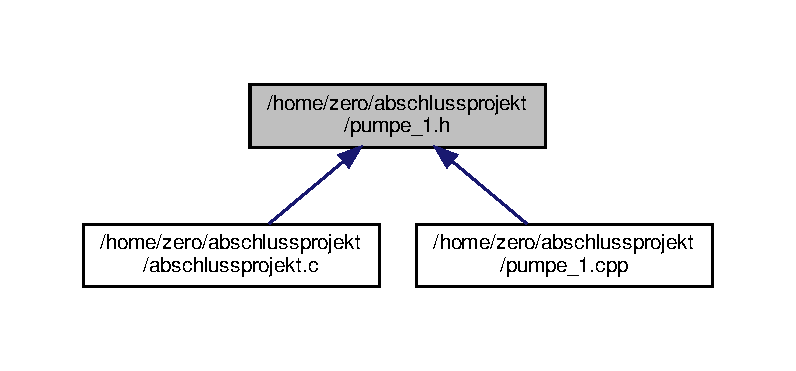
\includegraphics[width=350pt]{pumpe__1_8h__dep__incl}
\end{center}
\end{figure}
\subsection*{Funktionen}
\begin{DoxyCompactItemize}
\item 
void \hyperlink{pumpe__1_8h_ad672a4455a5f5c803b5fd5ad87a41aa0}{pumpen\+\_\+1} (void)
\begin{DoxyCompactList}\small\item\em Zustandsautomat Pumpe 1 ///. \end{DoxyCompactList}\end{DoxyCompactItemize}


\subsection{Dokumentation der Funktionen}
\mbox{\Hypertarget{pumpe__1_8h_ad672a4455a5f5c803b5fd5ad87a41aa0}\label{pumpe__1_8h_ad672a4455a5f5c803b5fd5ad87a41aa0}} 
\index{pumpe\+\_\+1.\+h@{pumpe\+\_\+1.\+h}!pumpen\+\_\+1@{pumpen\+\_\+1}}
\index{pumpen\+\_\+1@{pumpen\+\_\+1}!pumpe\+\_\+1.\+h@{pumpe\+\_\+1.\+h}}
\subsubsection{\texorpdfstring{pumpen\+\_\+1()}{pumpen\_1()}}
{\footnotesize\ttfamily void pumpen\+\_\+1 (\begin{DoxyParamCaption}\item[{void}]{ }\end{DoxyParamCaption})}



Zustandsautomat Pumpe 1 ///. 



Definiert in Zeile 16 der Datei pumpe\+\_\+1.\+cpp.


\hypertarget{pumpe__2_8cpp}{}\section{/home/zero/abschlussprojekt/pumpe\+\_\+2.cpp-\/\+Dateireferenz}
\label{pumpe__2_8cpp}\index{/home/zero/abschlussprojekt/pumpe\+\_\+2.\+cpp@{/home/zero/abschlussprojekt/pumpe\+\_\+2.\+cpp}}
{\ttfamily \#include $<$Arduino.\+h$>$}\newline
{\ttfamily \#include \char`\"{}makros.\+h\char`\"{}}\newline
{\ttfamily \#include \char`\"{}tuer\+\_\+zu.\+h\char`\"{}}\newline
{\ttfamily \#include \char`\"{}pumpe\+\_\+2.\+h\char`\"{}}\newline
Include-\/\+Abhängigkeitsdiagramm für pumpe\+\_\+2.\+cpp\+:
\nopagebreak
\begin{figure}[H]
\begin{center}
\leavevmode
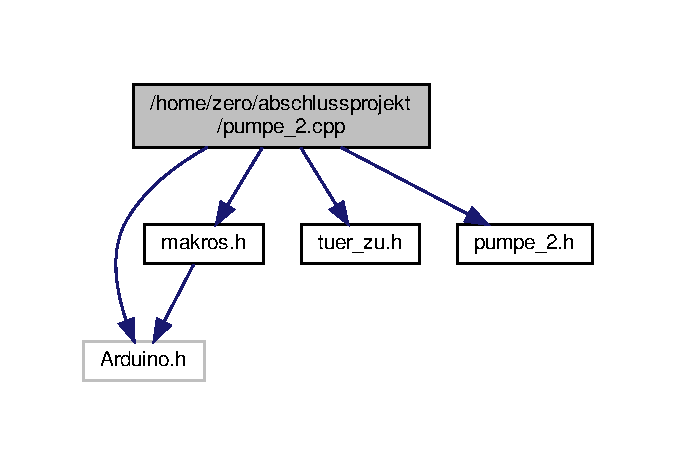
\includegraphics[width=325pt]{pumpe__2_8cpp__incl}
\end{center}
\end{figure}
\subsection*{Funktionen}
\begin{DoxyCompactItemize}
\item 
void \hyperlink{pumpe__2_8cpp_ab5052e43d029ec1d5b2899be0135e45c}{pumpen\+\_\+2} ()
\begin{DoxyCompactList}\small\item\em Zustandsautomat Pumpe 2 ///. \end{DoxyCompactList}\end{DoxyCompactItemize}
\subsection*{Variablen}
\begin{DoxyCompactItemize}
\item 
int \hyperlink{pumpe__2_8cpp_aacdbec939adcfa404b8c42b2e064b110}{hum\+\_\+erde\+\_\+2\+\_\+adc}
\item 
int \hyperlink{pumpe__2_8cpp_a11941af86181c1d0476b4bad92345dee}{limit\+\_\+feuchte\+\_\+2\+\_\+adc}
\item 
unsigned long \hyperlink{pumpe__2_8cpp_a6ba123b4db543f23167f7579070cb078}{t0\+\_\+pumpe\+\_\+2}
\item 
unsigned long \hyperlink{pumpe__2_8cpp_aa162b2945b33207aaa0e405a04e21049}{dt\+\_\+pumpendauer\+\_\+2\+\_\+ms} = 5000
\item 
unsigned long \hyperlink{pumpe__2_8cpp_ae43a32686ec363ab79244493e815eb1a}{t0\+\_\+durchfeuchtung\+\_\+2}
\item 
unsigned long \hyperlink{pumpe__2_8cpp_ad4082581e55599e78402c968aa6fd220}{dt\+\_\+warten\+\_\+durchfeuchtung\+\_\+2\+\_\+ms} = 10000
\item 
int \hyperlink{pumpe__2_8cpp_ae5d230a4da9cb370063e945d94d7043a}{zustand\+\_\+2} = \hyperlink{makros_8h_acd99f73b20037e5fcba7a4a031e0f320}{zustand\+\_\+warten\+\_\+zu\+\_\+trocken}
\end{DoxyCompactItemize}


\subsection{Dokumentation der Funktionen}
\mbox{\Hypertarget{pumpe__2_8cpp_ab5052e43d029ec1d5b2899be0135e45c}\label{pumpe__2_8cpp_ab5052e43d029ec1d5b2899be0135e45c}} 
\index{pumpe\+\_\+2.\+cpp@{pumpe\+\_\+2.\+cpp}!pumpen\+\_\+2@{pumpen\+\_\+2}}
\index{pumpen\+\_\+2@{pumpen\+\_\+2}!pumpe\+\_\+2.\+cpp@{pumpe\+\_\+2.\+cpp}}
\subsubsection{\texorpdfstring{pumpen\+\_\+2()}{pumpen\_2()}}
{\footnotesize\ttfamily void pumpen\+\_\+2 (\begin{DoxyParamCaption}\item[{void}]{ }\end{DoxyParamCaption})}



Zustandsautomat Pumpe 2 ///. 



Definiert in Zeile 16 der Datei pumpe\+\_\+2.\+cpp.



\subsection{Variablen-\/\+Dokumentation}
\mbox{\Hypertarget{pumpe__2_8cpp_aa162b2945b33207aaa0e405a04e21049}\label{pumpe__2_8cpp_aa162b2945b33207aaa0e405a04e21049}} 
\index{pumpe\+\_\+2.\+cpp@{pumpe\+\_\+2.\+cpp}!dt\+\_\+pumpendauer\+\_\+2\+\_\+ms@{dt\+\_\+pumpendauer\+\_\+2\+\_\+ms}}
\index{dt\+\_\+pumpendauer\+\_\+2\+\_\+ms@{dt\+\_\+pumpendauer\+\_\+2\+\_\+ms}!pumpe\+\_\+2.\+cpp@{pumpe\+\_\+2.\+cpp}}
\subsubsection{\texorpdfstring{dt\+\_\+pumpendauer\+\_\+2\+\_\+ms}{dt\_pumpendauer\_2\_ms}}
{\footnotesize\ttfamily unsigned long dt\+\_\+pumpendauer\+\_\+2\+\_\+ms = 5000}



Definiert in Zeile 10 der Datei pumpe\+\_\+2.\+cpp.

\mbox{\Hypertarget{pumpe__2_8cpp_ad4082581e55599e78402c968aa6fd220}\label{pumpe__2_8cpp_ad4082581e55599e78402c968aa6fd220}} 
\index{pumpe\+\_\+2.\+cpp@{pumpe\+\_\+2.\+cpp}!dt\+\_\+warten\+\_\+durchfeuchtung\+\_\+2\+\_\+ms@{dt\+\_\+warten\+\_\+durchfeuchtung\+\_\+2\+\_\+ms}}
\index{dt\+\_\+warten\+\_\+durchfeuchtung\+\_\+2\+\_\+ms@{dt\+\_\+warten\+\_\+durchfeuchtung\+\_\+2\+\_\+ms}!pumpe\+\_\+2.\+cpp@{pumpe\+\_\+2.\+cpp}}
\subsubsection{\texorpdfstring{dt\+\_\+warten\+\_\+durchfeuchtung\+\_\+2\+\_\+ms}{dt\_warten\_durchfeuchtung\_2\_ms}}
{\footnotesize\ttfamily unsigned long dt\+\_\+warten\+\_\+durchfeuchtung\+\_\+2\+\_\+ms = 10000}



Definiert in Zeile 12 der Datei pumpe\+\_\+2.\+cpp.

\mbox{\Hypertarget{pumpe__2_8cpp_aacdbec939adcfa404b8c42b2e064b110}\label{pumpe__2_8cpp_aacdbec939adcfa404b8c42b2e064b110}} 
\index{pumpe\+\_\+2.\+cpp@{pumpe\+\_\+2.\+cpp}!hum\+\_\+erde\+\_\+2\+\_\+adc@{hum\+\_\+erde\+\_\+2\+\_\+adc}}
\index{hum\+\_\+erde\+\_\+2\+\_\+adc@{hum\+\_\+erde\+\_\+2\+\_\+adc}!pumpe\+\_\+2.\+cpp@{pumpe\+\_\+2.\+cpp}}
\subsubsection{\texorpdfstring{hum\+\_\+erde\+\_\+2\+\_\+adc}{hum\_erde\_2\_adc}}
{\footnotesize\ttfamily int hum\+\_\+erde\+\_\+2\+\_\+adc}



Definiert in Zeile 47 der Datei abschlussprojekt.\+c.

\mbox{\Hypertarget{pumpe__2_8cpp_a11941af86181c1d0476b4bad92345dee}\label{pumpe__2_8cpp_a11941af86181c1d0476b4bad92345dee}} 
\index{pumpe\+\_\+2.\+cpp@{pumpe\+\_\+2.\+cpp}!limit\+\_\+feuchte\+\_\+2\+\_\+adc@{limit\+\_\+feuchte\+\_\+2\+\_\+adc}}
\index{limit\+\_\+feuchte\+\_\+2\+\_\+adc@{limit\+\_\+feuchte\+\_\+2\+\_\+adc}!pumpe\+\_\+2.\+cpp@{pumpe\+\_\+2.\+cpp}}
\subsubsection{\texorpdfstring{limit\+\_\+feuchte\+\_\+2\+\_\+adc}{limit\_feuchte\_2\_adc}}
{\footnotesize\ttfamily int limit\+\_\+feuchte\+\_\+2\+\_\+adc}



Definiert in Zeile 53 der Datei abschlussprojekt.\+c.

\mbox{\Hypertarget{pumpe__2_8cpp_ae43a32686ec363ab79244493e815eb1a}\label{pumpe__2_8cpp_ae43a32686ec363ab79244493e815eb1a}} 
\index{pumpe\+\_\+2.\+cpp@{pumpe\+\_\+2.\+cpp}!t0\+\_\+durchfeuchtung\+\_\+2@{t0\+\_\+durchfeuchtung\+\_\+2}}
\index{t0\+\_\+durchfeuchtung\+\_\+2@{t0\+\_\+durchfeuchtung\+\_\+2}!pumpe\+\_\+2.\+cpp@{pumpe\+\_\+2.\+cpp}}
\subsubsection{\texorpdfstring{t0\+\_\+durchfeuchtung\+\_\+2}{t0\_durchfeuchtung\_2}}
{\footnotesize\ttfamily unsigned long t0\+\_\+durchfeuchtung\+\_\+2}



Definiert in Zeile 11 der Datei pumpe\+\_\+2.\+cpp.

\mbox{\Hypertarget{pumpe__2_8cpp_a6ba123b4db543f23167f7579070cb078}\label{pumpe__2_8cpp_a6ba123b4db543f23167f7579070cb078}} 
\index{pumpe\+\_\+2.\+cpp@{pumpe\+\_\+2.\+cpp}!t0\+\_\+pumpe\+\_\+2@{t0\+\_\+pumpe\+\_\+2}}
\index{t0\+\_\+pumpe\+\_\+2@{t0\+\_\+pumpe\+\_\+2}!pumpe\+\_\+2.\+cpp@{pumpe\+\_\+2.\+cpp}}
\subsubsection{\texorpdfstring{t0\+\_\+pumpe\+\_\+2}{t0\_pumpe\_2}}
{\footnotesize\ttfamily unsigned long t0\+\_\+pumpe\+\_\+2}



Definiert in Zeile 9 der Datei pumpe\+\_\+2.\+cpp.

\mbox{\Hypertarget{pumpe__2_8cpp_ae5d230a4da9cb370063e945d94d7043a}\label{pumpe__2_8cpp_ae5d230a4da9cb370063e945d94d7043a}} 
\index{pumpe\+\_\+2.\+cpp@{pumpe\+\_\+2.\+cpp}!zustand\+\_\+2@{zustand\+\_\+2}}
\index{zustand\+\_\+2@{zustand\+\_\+2}!pumpe\+\_\+2.\+cpp@{pumpe\+\_\+2.\+cpp}}
\subsubsection{\texorpdfstring{zustand\+\_\+2}{zustand\_2}}
{\footnotesize\ttfamily int zustand\+\_\+2 = \hyperlink{makros_8h_acd99f73b20037e5fcba7a4a031e0f320}{zustand\+\_\+warten\+\_\+zu\+\_\+trocken}}



Definiert in Zeile 14 der Datei pumpe\+\_\+2.\+cpp.


\hypertarget{pumpe__2_8h}{}\section{/home/zero/abschlussprojekt/pumpe\+\_\+2.h-\/\+Dateireferenz}
\label{pumpe__2_8h}\index{/home/zero/abschlussprojekt/pumpe\+\_\+2.\+h@{/home/zero/abschlussprojekt/pumpe\+\_\+2.\+h}}
Dieser Graph zeigt, welche Datei direkt oder indirekt diese Datei enthält\+:
\nopagebreak
\begin{figure}[H]
\begin{center}
\leavevmode
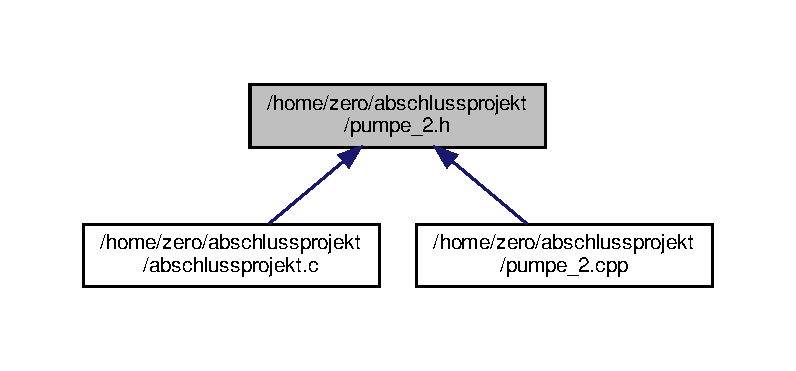
\includegraphics[width=350pt]{pumpe__2_8h__dep__incl}
\end{center}
\end{figure}
\subsection*{Funktionen}
\begin{DoxyCompactItemize}
\item 
void \hyperlink{pumpe__2_8h_a754bd6f3d38e83cc0365704a45bf8f37}{pumpen\+\_\+2} (void)
\begin{DoxyCompactList}\small\item\em Zustandsautomat Pumpe 2 ///. \end{DoxyCompactList}\end{DoxyCompactItemize}


\subsection{Dokumentation der Funktionen}
\mbox{\Hypertarget{pumpe__2_8h_a754bd6f3d38e83cc0365704a45bf8f37}\label{pumpe__2_8h_a754bd6f3d38e83cc0365704a45bf8f37}} 
\index{pumpe\+\_\+2.\+h@{pumpe\+\_\+2.\+h}!pumpen\+\_\+2@{pumpen\+\_\+2}}
\index{pumpen\+\_\+2@{pumpen\+\_\+2}!pumpe\+\_\+2.\+h@{pumpe\+\_\+2.\+h}}
\subsubsection{\texorpdfstring{pumpen\+\_\+2()}{pumpen\_2()}}
{\footnotesize\ttfamily void pumpen\+\_\+2 (\begin{DoxyParamCaption}\item[{void}]{ }\end{DoxyParamCaption})}



Zustandsautomat Pumpe 2 ///. 



Definiert in Zeile 16 der Datei pumpe\+\_\+2.\+cpp.


\hypertarget{tuer__zu_8cpp}{}\section{/home/zero/abschlussprojekt/tuer\+\_\+zu.cpp-\/\+Dateireferenz}
\label{tuer__zu_8cpp}\index{/home/zero/abschlussprojekt/tuer\+\_\+zu.\+cpp@{/home/zero/abschlussprojekt/tuer\+\_\+zu.\+cpp}}
{\ttfamily \#include $<$Arduino.\+h$>$}\newline
{\ttfamily \#include \char`\"{}makros.\+h\char`\"{}}\newline
{\ttfamily \#include \char`\"{}tuer\+\_\+zu.\+h\char`\"{}}\newline
Include-\/\+Abhängigkeitsdiagramm für tuer\+\_\+zu.\+cpp\+:
\nopagebreak
\begin{figure}[H]
\begin{center}
\leavevmode
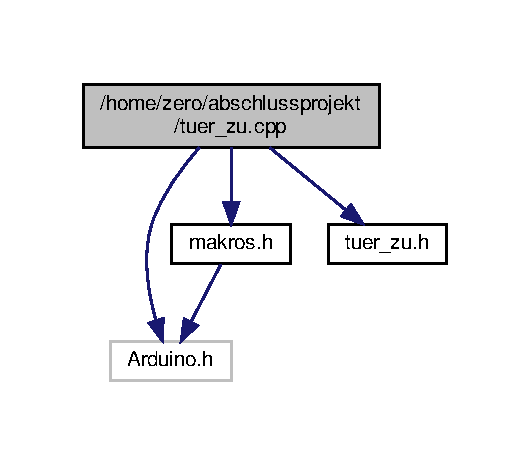
\includegraphics[width=255pt]{tuer__zu_8cpp__incl}
\end{center}
\end{figure}
\subsection*{Funktionen}
\begin{DoxyCompactItemize}
\item 
bool \hyperlink{tuer__zu_8cpp_a204dcf18a43cbaf756753c4de7bc10b4}{tuer\+\_\+zu} ()
\begin{DoxyCompactList}\small\item\em Auswertung des R\+E\+E\+D-\/\+Kontaktes ///. \end{DoxyCompactList}\end{DoxyCompactItemize}


\subsection{Dokumentation der Funktionen}
\mbox{\Hypertarget{tuer__zu_8cpp_a204dcf18a43cbaf756753c4de7bc10b4}\label{tuer__zu_8cpp_a204dcf18a43cbaf756753c4de7bc10b4}} 
\index{tuer\+\_\+zu.\+cpp@{tuer\+\_\+zu.\+cpp}!tuer\+\_\+zu@{tuer\+\_\+zu}}
\index{tuer\+\_\+zu@{tuer\+\_\+zu}!tuer\+\_\+zu.\+cpp@{tuer\+\_\+zu.\+cpp}}
\subsubsection{\texorpdfstring{tuer\+\_\+zu()}{tuer\_zu()}}
{\footnotesize\ttfamily bool tuer\+\_\+zu (\begin{DoxyParamCaption}{ }\end{DoxyParamCaption})}



Auswertung des R\+E\+E\+D-\/\+Kontaktes ///. 



Definiert in Zeile 8 der Datei tuer\+\_\+zu.\+cpp.


\hypertarget{tuer__zu_8h}{}\section{/home/zero/abschlussprojekt/tuer\+\_\+zu.h-\/\+Dateireferenz}
\label{tuer__zu_8h}\index{/home/zero/abschlussprojekt/tuer\+\_\+zu.\+h@{/home/zero/abschlussprojekt/tuer\+\_\+zu.\+h}}
Dieser Graph zeigt, welche Datei direkt oder indirekt diese Datei enthält\+:
\nopagebreak
\begin{figure}[H]
\begin{center}
\leavevmode
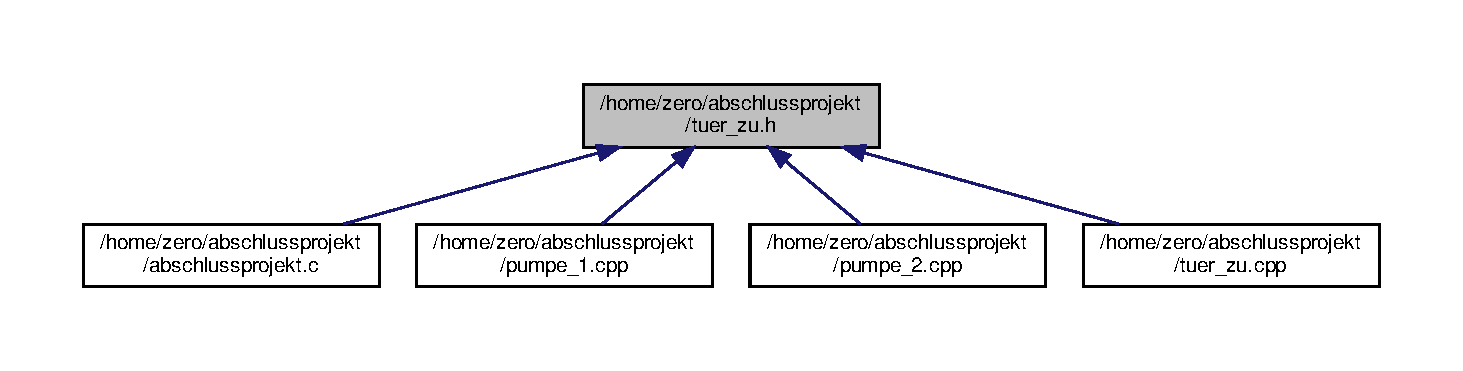
\includegraphics[width=350pt]{tuer__zu_8h__dep__incl}
\end{center}
\end{figure}
\subsection*{Funktionen}
\begin{DoxyCompactItemize}
\item 
bool \hyperlink{tuer__zu_8h_a204dcf18a43cbaf756753c4de7bc10b4}{tuer\+\_\+zu} ()
\begin{DoxyCompactList}\small\item\em Auswertung des R\+E\+E\+D-\/\+Kontaktes ///. \end{DoxyCompactList}\end{DoxyCompactItemize}


\subsection{Dokumentation der Funktionen}
\mbox{\Hypertarget{tuer__zu_8h_a204dcf18a43cbaf756753c4de7bc10b4}\label{tuer__zu_8h_a204dcf18a43cbaf756753c4de7bc10b4}} 
\index{tuer\+\_\+zu.\+h@{tuer\+\_\+zu.\+h}!tuer\+\_\+zu@{tuer\+\_\+zu}}
\index{tuer\+\_\+zu@{tuer\+\_\+zu}!tuer\+\_\+zu.\+h@{tuer\+\_\+zu.\+h}}
\subsubsection{\texorpdfstring{tuer\+\_\+zu()}{tuer\_zu()}}
{\footnotesize\ttfamily bool tuer\+\_\+zu (\begin{DoxyParamCaption}{ }\end{DoxyParamCaption})}



Auswertung des R\+E\+E\+D-\/\+Kontaktes ///. 



Definiert in Zeile 8 der Datei tuer\+\_\+zu.\+cpp.


\hypertarget{update__lcd_8h}{}\section{/home/zero/abschlussprojekt/update\+\_\+lcd.h-\/\+Dateireferenz}
\label{update__lcd_8h}\index{/home/zero/abschlussprojekt/update\+\_\+lcd.\+h@{/home/zero/abschlussprojekt/update\+\_\+lcd.\+h}}
{\ttfamily \#include $<$Arduino.\+h$>$}\newline
{\ttfamily \#include $<$Liquid\+Crystal\+\_\+\+I2\+C.\+h$>$}\newline
{\ttfamily \#include \char`\"{}make\+\_\+string.\+h\char`\"{}}\newline
Include-\/\+Abhängigkeitsdiagramm für update\+\_\+lcd.\+h\+:
\nopagebreak
\begin{figure}[H]
\begin{center}
\leavevmode
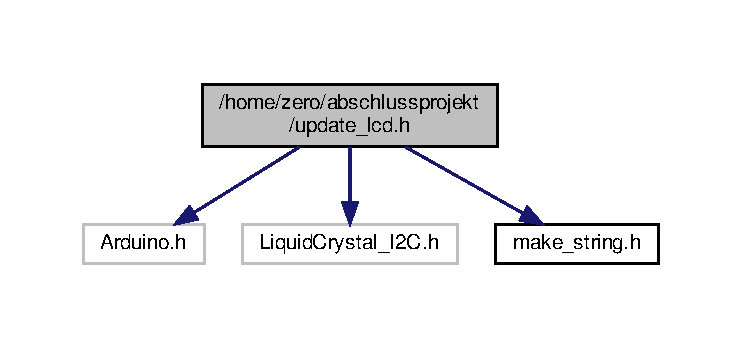
\includegraphics[width=350pt]{update__lcd_8h__incl}
\end{center}
\end{figure}
Dieser Graph zeigt, welche Datei direkt oder indirekt diese Datei enthält\+:
\nopagebreak
\begin{figure}[H]
\begin{center}
\leavevmode
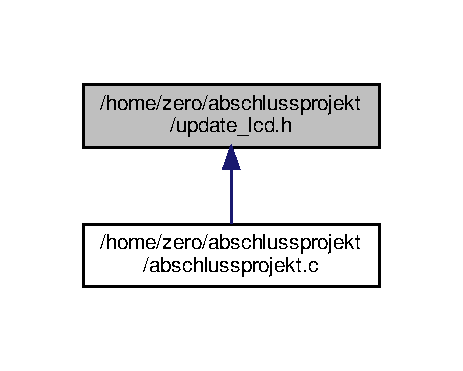
\includegraphics[width=222pt]{update__lcd_8h__dep__incl}
\end{center}
\end{figure}
\subsection*{Funktionen}
\begin{DoxyCompactItemize}
\item 
Liquid\+Crystal\+\_\+\+I2C \hyperlink{update__lcd_8h_a7392e8043ba37d68cf0d13e0264acd85}{lcd} (0x3\+F, 20, 4)
\item 
void \hyperlink{update__lcd_8h_a23904742a80994988f92b99487c299ca}{update\+\_\+lcd} (int nr\+\_\+display, int \hyperlink{update__messwerte_8h_a0e6f058da75dead800f4a33e63586703}{temp\+\_\+luft\+\_\+C}, int \hyperlink{update__messwerte_8h_ac9fcb87eca48e4002731015e004966ef}{hum\+\_\+luft}, int \hyperlink{update__messwerte_8h_afa416e7460cf043207be351d750b97fe}{hum\+\_\+erde\+\_\+1\+\_\+adc}, int \hyperlink{update__messwerte_8h_aacdbec939adcfa404b8c42b2e064b110}{hum\+\_\+erde\+\_\+2\+\_\+adc}, int \hyperlink{update__limits_8cpp_abb1c509cfb119e70585771234accdc4c}{limit\+\_\+feuchte\+\_\+1\+\_\+adc}, int \hyperlink{update__limits_8cpp_a11941af86181c1d0476b4bad92345dee}{limit\+\_\+feuchte\+\_\+2\+\_\+adc}, int \hyperlink{update__limits_8cpp_a8f0ffb4ec25253a324ab4dac6d3cf1c4}{limit\+\_\+temp\+\_\+adc}, int \hyperlink{update__limits_8cpp_a3f6dd9ed3b997c063d7c90a38a69ab3a}{limit\+\_\+luefter\+\_\+adc})
\end{DoxyCompactItemize}


\subsection{Dokumentation der Funktionen}
\mbox{\Hypertarget{update__lcd_8h_a7392e8043ba37d68cf0d13e0264acd85}\label{update__lcd_8h_a7392e8043ba37d68cf0d13e0264acd85}} 
\index{update\+\_\+lcd.\+h@{update\+\_\+lcd.\+h}!lcd@{lcd}}
\index{lcd@{lcd}!update\+\_\+lcd.\+h@{update\+\_\+lcd.\+h}}
\subsubsection{\texorpdfstring{lcd()}{lcd()}}
{\footnotesize\ttfamily Liquid\+Crystal\+\_\+\+I2C lcd (\begin{DoxyParamCaption}\item[{0x3F}]{,  }\item[{20}]{,  }\item[{4}]{ }\end{DoxyParamCaption})}

\mbox{\Hypertarget{update__lcd_8h_a23904742a80994988f92b99487c299ca}\label{update__lcd_8h_a23904742a80994988f92b99487c299ca}} 
\index{update\+\_\+lcd.\+h@{update\+\_\+lcd.\+h}!update\+\_\+lcd@{update\+\_\+lcd}}
\index{update\+\_\+lcd@{update\+\_\+lcd}!update\+\_\+lcd.\+h@{update\+\_\+lcd.\+h}}
\subsubsection{\texorpdfstring{update\+\_\+lcd()}{update\_lcd()}}
{\footnotesize\ttfamily void update\+\_\+lcd (\begin{DoxyParamCaption}\item[{int}]{nr\+\_\+display,  }\item[{int}]{temp\+\_\+luft\+\_\+C,  }\item[{int}]{hum\+\_\+luft,  }\item[{int}]{hum\+\_\+erde\+\_\+1\+\_\+adc,  }\item[{int}]{hum\+\_\+erde\+\_\+2\+\_\+adc,  }\item[{int}]{limit\+\_\+feuchte\+\_\+1\+\_\+adc,  }\item[{int}]{limit\+\_\+feuchte\+\_\+2\+\_\+adc,  }\item[{int}]{limit\+\_\+temp\+\_\+adc,  }\item[{int}]{limit\+\_\+luefter\+\_\+adc }\end{DoxyParamCaption})}



Definiert in Zeile 8 der Datei update\+\_\+lcd.\+h.


\hypertarget{update__limits_8cpp}{}\section{/home/zero/abschlussprojekt/update\+\_\+limits.cpp-\/\+Dateireferenz}
\label{update__limits_8cpp}\index{/home/zero/abschlussprojekt/update\+\_\+limits.\+cpp@{/home/zero/abschlussprojekt/update\+\_\+limits.\+cpp}}
{\ttfamily \#include $<$Arduino.\+h$>$}\newline
{\ttfamily \#include \char`\"{}makros.\+h\char`\"{}}\newline
{\ttfamily \#include \char`\"{}update\+\_\+limits.\+h\char`\"{}}\newline
Include-\/\+Abhängigkeitsdiagramm für update\+\_\+limits.\+cpp\+:
\nopagebreak
\begin{figure}[H]
\begin{center}
\leavevmode
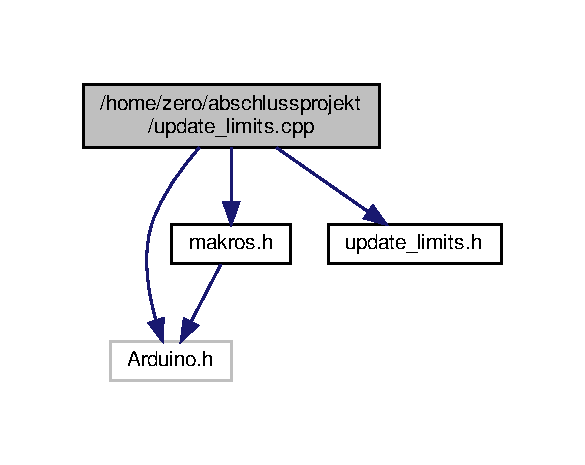
\includegraphics[width=281pt]{update__limits_8cpp__incl}
\end{center}
\end{figure}
\subsection*{Funktionen}
\begin{DoxyCompactItemize}
\item 
void \hyperlink{update__limits_8cpp_a1efb14d12b812e3a0f08188dbaeccc5e}{update\+\_\+limits} ()
\begin{DoxyCompactList}\small\item\em aktualisieren der Schwellenwerte /// \end{DoxyCompactList}\end{DoxyCompactItemize}
\subsection*{Variablen}
\begin{DoxyCompactItemize}
\item 
int \hyperlink{update__limits_8cpp_abb1c509cfb119e70585771234accdc4c}{limit\+\_\+feuchte\+\_\+1\+\_\+adc}
\item 
int \hyperlink{update__limits_8cpp_a11941af86181c1d0476b4bad92345dee}{limit\+\_\+feuchte\+\_\+2\+\_\+adc}
\item 
int \hyperlink{update__limits_8cpp_a8f0ffb4ec25253a324ab4dac6d3cf1c4}{limit\+\_\+temp\+\_\+adc}
\item 
int \hyperlink{update__limits_8cpp_a7af3ab4da71f5b8ce8c0d93640690817}{limit\+\_\+temp\+\_\+C}
\item 
int \hyperlink{update__limits_8cpp_a3f6dd9ed3b997c063d7c90a38a69ab3a}{limit\+\_\+luefter\+\_\+adc}
\item 
int \hyperlink{update__limits_8cpp_a27d916670e311d9e7881ebdc4807e0f5}{limit\+\_\+luefter\+\_\+C}
\end{DoxyCompactItemize}


\subsection{Dokumentation der Funktionen}
\mbox{\Hypertarget{update__limits_8cpp_a1efb14d12b812e3a0f08188dbaeccc5e}\label{update__limits_8cpp_a1efb14d12b812e3a0f08188dbaeccc5e}} 
\index{update\+\_\+limits.\+cpp@{update\+\_\+limits.\+cpp}!update\+\_\+limits@{update\+\_\+limits}}
\index{update\+\_\+limits@{update\+\_\+limits}!update\+\_\+limits.\+cpp@{update\+\_\+limits.\+cpp}}
\subsubsection{\texorpdfstring{update\+\_\+limits()}{update\_limits()}}
{\footnotesize\ttfamily void update\+\_\+limits (\begin{DoxyParamCaption}\item[{void}]{ }\end{DoxyParamCaption})}



aktualisieren der Schwellenwerte /// 



Definiert in Zeile 13 der Datei update\+\_\+limits.\+cpp.



\subsection{Variablen-\/\+Dokumentation}
\mbox{\Hypertarget{update__limits_8cpp_abb1c509cfb119e70585771234accdc4c}\label{update__limits_8cpp_abb1c509cfb119e70585771234accdc4c}} 
\index{update\+\_\+limits.\+cpp@{update\+\_\+limits.\+cpp}!limit\+\_\+feuchte\+\_\+1\+\_\+adc@{limit\+\_\+feuchte\+\_\+1\+\_\+adc}}
\index{limit\+\_\+feuchte\+\_\+1\+\_\+adc@{limit\+\_\+feuchte\+\_\+1\+\_\+adc}!update\+\_\+limits.\+cpp@{update\+\_\+limits.\+cpp}}
\subsubsection{\texorpdfstring{limit\+\_\+feuchte\+\_\+1\+\_\+adc}{limit\_feuchte\_1\_adc}}
{\footnotesize\ttfamily int limit\+\_\+feuchte\+\_\+1\+\_\+adc}



Definiert in Zeile 52 der Datei abschlussprojekt.\+c.

\mbox{\Hypertarget{update__limits_8cpp_a11941af86181c1d0476b4bad92345dee}\label{update__limits_8cpp_a11941af86181c1d0476b4bad92345dee}} 
\index{update\+\_\+limits.\+cpp@{update\+\_\+limits.\+cpp}!limit\+\_\+feuchte\+\_\+2\+\_\+adc@{limit\+\_\+feuchte\+\_\+2\+\_\+adc}}
\index{limit\+\_\+feuchte\+\_\+2\+\_\+adc@{limit\+\_\+feuchte\+\_\+2\+\_\+adc}!update\+\_\+limits.\+cpp@{update\+\_\+limits.\+cpp}}
\subsubsection{\texorpdfstring{limit\+\_\+feuchte\+\_\+2\+\_\+adc}{limit\_feuchte\_2\_adc}}
{\footnotesize\ttfamily int limit\+\_\+feuchte\+\_\+2\+\_\+adc}



Definiert in Zeile 53 der Datei abschlussprojekt.\+c.

\mbox{\Hypertarget{update__limits_8cpp_a3f6dd9ed3b997c063d7c90a38a69ab3a}\label{update__limits_8cpp_a3f6dd9ed3b997c063d7c90a38a69ab3a}} 
\index{update\+\_\+limits.\+cpp@{update\+\_\+limits.\+cpp}!limit\+\_\+luefter\+\_\+adc@{limit\+\_\+luefter\+\_\+adc}}
\index{limit\+\_\+luefter\+\_\+adc@{limit\+\_\+luefter\+\_\+adc}!update\+\_\+limits.\+cpp@{update\+\_\+limits.\+cpp}}
\subsubsection{\texorpdfstring{limit\+\_\+luefter\+\_\+adc}{limit\_luefter\_adc}}
{\footnotesize\ttfamily int limit\+\_\+luefter\+\_\+adc}



Definiert in Zeile 56 der Datei abschlussprojekt.\+c.

\mbox{\Hypertarget{update__limits_8cpp_a27d916670e311d9e7881ebdc4807e0f5}\label{update__limits_8cpp_a27d916670e311d9e7881ebdc4807e0f5}} 
\index{update\+\_\+limits.\+cpp@{update\+\_\+limits.\+cpp}!limit\+\_\+luefter\+\_\+C@{limit\+\_\+luefter\+\_\+C}}
\index{limit\+\_\+luefter\+\_\+C@{limit\+\_\+luefter\+\_\+C}!update\+\_\+limits.\+cpp@{update\+\_\+limits.\+cpp}}
\subsubsection{\texorpdfstring{limit\+\_\+luefter\+\_\+C}{limit\_luefter\_C}}
{\footnotesize\ttfamily int limit\+\_\+luefter\+\_\+C}



Definiert in Zeile 57 der Datei abschlussprojekt.\+c.

\mbox{\Hypertarget{update__limits_8cpp_a8f0ffb4ec25253a324ab4dac6d3cf1c4}\label{update__limits_8cpp_a8f0ffb4ec25253a324ab4dac6d3cf1c4}} 
\index{update\+\_\+limits.\+cpp@{update\+\_\+limits.\+cpp}!limit\+\_\+temp\+\_\+adc@{limit\+\_\+temp\+\_\+adc}}
\index{limit\+\_\+temp\+\_\+adc@{limit\+\_\+temp\+\_\+adc}!update\+\_\+limits.\+cpp@{update\+\_\+limits.\+cpp}}
\subsubsection{\texorpdfstring{limit\+\_\+temp\+\_\+adc}{limit\_temp\_adc}}
{\footnotesize\ttfamily int limit\+\_\+temp\+\_\+adc}



Definiert in Zeile 54 der Datei abschlussprojekt.\+c.

\mbox{\Hypertarget{update__limits_8cpp_a7af3ab4da71f5b8ce8c0d93640690817}\label{update__limits_8cpp_a7af3ab4da71f5b8ce8c0d93640690817}} 
\index{update\+\_\+limits.\+cpp@{update\+\_\+limits.\+cpp}!limit\+\_\+temp\+\_\+C@{limit\+\_\+temp\+\_\+C}}
\index{limit\+\_\+temp\+\_\+C@{limit\+\_\+temp\+\_\+C}!update\+\_\+limits.\+cpp@{update\+\_\+limits.\+cpp}}
\subsubsection{\texorpdfstring{limit\+\_\+temp\+\_\+C}{limit\_temp\_C}}
{\footnotesize\ttfamily int limit\+\_\+temp\+\_\+C}



Definiert in Zeile 55 der Datei abschlussprojekt.\+c.


\hypertarget{update__limits_8h}{}\section{/home/zero/abschlussprojekt/update\+\_\+limits.h-\/\+Dateireferenz}
\label{update__limits_8h}\index{/home/zero/abschlussprojekt/update\+\_\+limits.\+h@{/home/zero/abschlussprojekt/update\+\_\+limits.\+h}}
Dieser Graph zeigt, welche Datei direkt oder indirekt diese Datei enthält\+:
\nopagebreak
\begin{figure}[H]
\begin{center}
\leavevmode
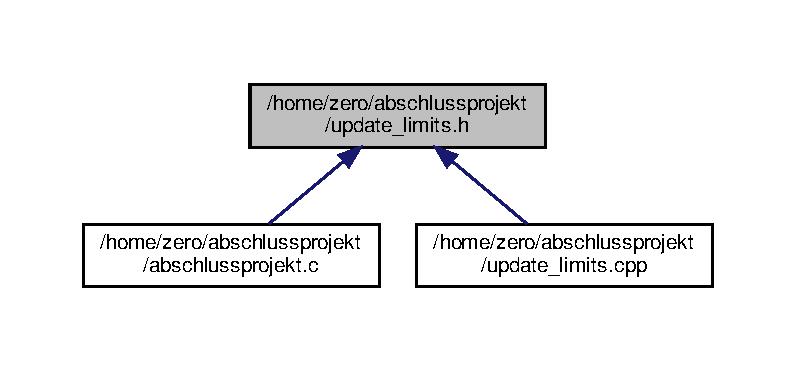
\includegraphics[width=350pt]{update__limits_8h__dep__incl}
\end{center}
\end{figure}
\subsection*{Funktionen}
\begin{DoxyCompactItemize}
\item 
void \hyperlink{update__limits_8h_aa626307640ddc7baa35c92ff1713e6bb}{update\+\_\+limits} (void)
\begin{DoxyCompactList}\small\item\em aktualisieren der Schwellenwerte /// \end{DoxyCompactList}\end{DoxyCompactItemize}


\subsection{Dokumentation der Funktionen}
\mbox{\Hypertarget{update__limits_8h_aa626307640ddc7baa35c92ff1713e6bb}\label{update__limits_8h_aa626307640ddc7baa35c92ff1713e6bb}} 
\index{update\+\_\+limits.\+h@{update\+\_\+limits.\+h}!update\+\_\+limits@{update\+\_\+limits}}
\index{update\+\_\+limits@{update\+\_\+limits}!update\+\_\+limits.\+h@{update\+\_\+limits.\+h}}
\subsubsection{\texorpdfstring{update\+\_\+limits()}{update\_limits()}}
{\footnotesize\ttfamily void update\+\_\+limits (\begin{DoxyParamCaption}\item[{void}]{ }\end{DoxyParamCaption})}



aktualisieren der Schwellenwerte /// 



Definiert in Zeile 13 der Datei update\+\_\+limits.\+cpp.


\hypertarget{update__messwerte_8h}{}\section{/home/zero/abschlussprojekt/update\+\_\+messwerte.h-\/\+Dateireferenz}
\label{update__messwerte_8h}\index{/home/zero/abschlussprojekt/update\+\_\+messwerte.\+h@{/home/zero/abschlussprojekt/update\+\_\+messwerte.\+h}}
{\ttfamily \#include $<$Arduino.\+h$>$}\newline
{\ttfamily \#include \char`\"{}makros.\+h\char`\"{}}\newline
{\ttfamily \#include \char`\"{}D\+H\+T.\+h\char`\"{}}\newline
Include-\/\+Abhängigkeitsdiagramm für update\+\_\+messwerte.\+h\+:
\nopagebreak
\begin{figure}[H]
\begin{center}
\leavevmode
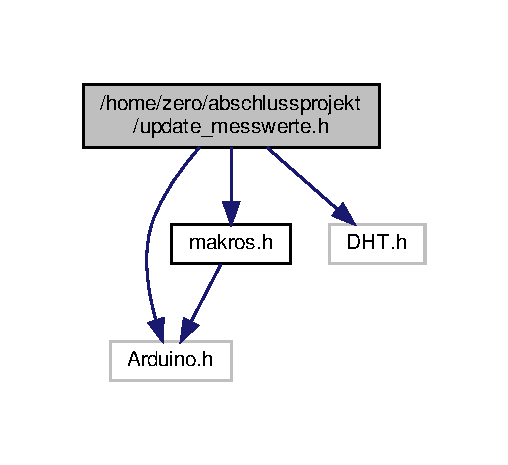
\includegraphics[width=244pt]{update__messwerte_8h__incl}
\end{center}
\end{figure}
Dieser Graph zeigt, welche Datei direkt oder indirekt diese Datei enthält\+:
\nopagebreak
\begin{figure}[H]
\begin{center}
\leavevmode
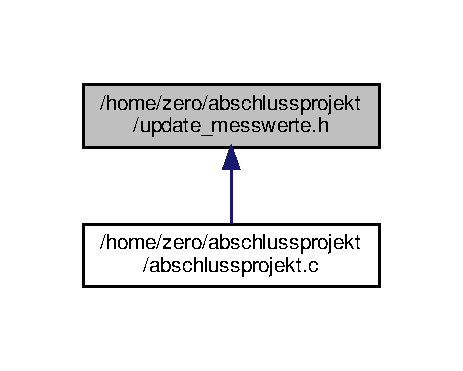
\includegraphics[width=222pt]{update__messwerte_8h__dep__incl}
\end{center}
\end{figure}
\subsection*{Funktionen}
\begin{DoxyCompactItemize}
\item 
D\+HT \hyperlink{update__messwerte_8h_a94f388d273b0cbe6d7f3c0d5817f688b}{dht} (\hyperlink{makros_8h_a9894c05769fdf48b3506408030591a65}{T\+E\+M\+P\+E\+R\+A\+T\+U\+R\+S\+E\+N\+S\+O\+R\+\_\+\+L\+U\+E\+F\+T\+ER}, \hyperlink{makros_8h_a2c509dba12bba99883a5be9341b7a0c5}{D\+H\+T\+T\+Y\+PE})
\item 
void \hyperlink{update__messwerte_8h_a992b1037e3565070916e60498c1a62ff}{update\+\_\+messwerte} ()
\end{DoxyCompactItemize}
\subsection*{Variablen}
\begin{DoxyCompactItemize}
\item 
int \hyperlink{update__messwerte_8h_afa416e7460cf043207be351d750b97fe}{hum\+\_\+erde\+\_\+1\+\_\+adc}
\item 
int \hyperlink{update__messwerte_8h_aacdbec939adcfa404b8c42b2e064b110}{hum\+\_\+erde\+\_\+2\+\_\+adc}
\item 
int \hyperlink{update__messwerte_8h_ac9fcb87eca48e4002731015e004966ef}{hum\+\_\+luft}
\item 
int \hyperlink{update__messwerte_8h_a0e6f058da75dead800f4a33e63586703}{temp\+\_\+luft\+\_\+C}
\end{DoxyCompactItemize}


\subsection{Dokumentation der Funktionen}
\mbox{\Hypertarget{update__messwerte_8h_a94f388d273b0cbe6d7f3c0d5817f688b}\label{update__messwerte_8h_a94f388d273b0cbe6d7f3c0d5817f688b}} 
\index{update\+\_\+messwerte.\+h@{update\+\_\+messwerte.\+h}!dht@{dht}}
\index{dht@{dht}!update\+\_\+messwerte.\+h@{update\+\_\+messwerte.\+h}}
\subsubsection{\texorpdfstring{dht()}{dht()}}
{\footnotesize\ttfamily D\+HT dht (\begin{DoxyParamCaption}\item[{\hyperlink{makros_8h_a9894c05769fdf48b3506408030591a65}{T\+E\+M\+P\+E\+R\+A\+T\+U\+R\+S\+E\+N\+S\+O\+R\+\_\+\+L\+U\+E\+F\+T\+ER}}]{,  }\item[{\hyperlink{makros_8h_a2c509dba12bba99883a5be9341b7a0c5}{D\+H\+T\+T\+Y\+PE}}]{ }\end{DoxyParamCaption})}

\mbox{\Hypertarget{update__messwerte_8h_a992b1037e3565070916e60498c1a62ff}\label{update__messwerte_8h_a992b1037e3565070916e60498c1a62ff}} 
\index{update\+\_\+messwerte.\+h@{update\+\_\+messwerte.\+h}!update\+\_\+messwerte@{update\+\_\+messwerte}}
\index{update\+\_\+messwerte@{update\+\_\+messwerte}!update\+\_\+messwerte.\+h@{update\+\_\+messwerte.\+h}}
\subsubsection{\texorpdfstring{update\+\_\+messwerte()}{update\_messwerte()}}
{\footnotesize\ttfamily void update\+\_\+messwerte (\begin{DoxyParamCaption}{ }\end{DoxyParamCaption})}



Definiert in Zeile 14 der Datei update\+\_\+messwerte.\+h.



\subsection{Variablen-\/\+Dokumentation}
\mbox{\Hypertarget{update__messwerte_8h_afa416e7460cf043207be351d750b97fe}\label{update__messwerte_8h_afa416e7460cf043207be351d750b97fe}} 
\index{update\+\_\+messwerte.\+h@{update\+\_\+messwerte.\+h}!hum\+\_\+erde\+\_\+1\+\_\+adc@{hum\+\_\+erde\+\_\+1\+\_\+adc}}
\index{hum\+\_\+erde\+\_\+1\+\_\+adc@{hum\+\_\+erde\+\_\+1\+\_\+adc}!update\+\_\+messwerte.\+h@{update\+\_\+messwerte.\+h}}
\subsubsection{\texorpdfstring{hum\+\_\+erde\+\_\+1\+\_\+adc}{hum\_erde\_1\_adc}}
{\footnotesize\ttfamily int hum\+\_\+erde\+\_\+1\+\_\+adc}



Definiert in Zeile 46 der Datei abschlussprojekt.\+c.

\mbox{\Hypertarget{update__messwerte_8h_aacdbec939adcfa404b8c42b2e064b110}\label{update__messwerte_8h_aacdbec939adcfa404b8c42b2e064b110}} 
\index{update\+\_\+messwerte.\+h@{update\+\_\+messwerte.\+h}!hum\+\_\+erde\+\_\+2\+\_\+adc@{hum\+\_\+erde\+\_\+2\+\_\+adc}}
\index{hum\+\_\+erde\+\_\+2\+\_\+adc@{hum\+\_\+erde\+\_\+2\+\_\+adc}!update\+\_\+messwerte.\+h@{update\+\_\+messwerte.\+h}}
\subsubsection{\texorpdfstring{hum\+\_\+erde\+\_\+2\+\_\+adc}{hum\_erde\_2\_adc}}
{\footnotesize\ttfamily int hum\+\_\+erde\+\_\+2\+\_\+adc}



Definiert in Zeile 47 der Datei abschlussprojekt.\+c.

\mbox{\Hypertarget{update__messwerte_8h_ac9fcb87eca48e4002731015e004966ef}\label{update__messwerte_8h_ac9fcb87eca48e4002731015e004966ef}} 
\index{update\+\_\+messwerte.\+h@{update\+\_\+messwerte.\+h}!hum\+\_\+luft@{hum\+\_\+luft}}
\index{hum\+\_\+luft@{hum\+\_\+luft}!update\+\_\+messwerte.\+h@{update\+\_\+messwerte.\+h}}
\subsubsection{\texorpdfstring{hum\+\_\+luft}{hum\_luft}}
{\footnotesize\ttfamily int hum\+\_\+luft}



Definiert in Zeile 48 der Datei abschlussprojekt.\+c.

\mbox{\Hypertarget{update__messwerte_8h_a0e6f058da75dead800f4a33e63586703}\label{update__messwerte_8h_a0e6f058da75dead800f4a33e63586703}} 
\index{update\+\_\+messwerte.\+h@{update\+\_\+messwerte.\+h}!temp\+\_\+luft\+\_\+C@{temp\+\_\+luft\+\_\+C}}
\index{temp\+\_\+luft\+\_\+C@{temp\+\_\+luft\+\_\+C}!update\+\_\+messwerte.\+h@{update\+\_\+messwerte.\+h}}
\subsubsection{\texorpdfstring{temp\+\_\+luft\+\_\+C}{temp\_luft\_C}}
{\footnotesize\ttfamily int temp\+\_\+luft\+\_\+C}



Definiert in Zeile 49 der Datei abschlussprojekt.\+c.


%--- End generated contents ---

% Index
\backmatter
\newpage
\phantomsection
\clearemptydoublepage
\addcontentsline{toc}{chapter}{Index}
\printindex

\end{document}
